\documentclass[11pt,a4paper,twocolumn]{article}

\usepackage[margin=1in]{geometry}
\usepackage{amsmath,amssymb}
\usepackage{graphicx}
\usepackage{booktabs}
\usepackage{array}
\usepackage{microtype}
\microtypesetup{expansion=false}
\usepackage{makecell}
\usepackage{longtable}
% Avoid "Infinite glue shrinkage" when longtable splits across pages (latex2e #1907).
\usepackage{etoolbox}
\makeatletter
\patchcmd{\LT@output}{\copy\LT@foot\vss}{%
  \copy\LT@foot\vskip 0pt plus \maxdimen minus \normalbaselineskip}{}{%
  \typeout{Warning: longtable infinite-glue patch failed}}
\patchcmd{\LT@output}{\copy\LT@foot\vss}{%
  \copy\LT@foot\vskip 0pt plus \maxdimen minus \normalbaselineskip}{}{%
  \typeout{Warning: longtable infinite-glue patch failed}}
\makeatother
\usepackage{url}
\usepackage{xurl}
\usepackage{float}
\usepackage{orcidlink}
\usepackage{hyperref}
\usepackage{cleveref}
\hypersetup{
  colorlinks=true,
  linkcolor=blue,
  citecolor=blue,
  urlcolor=blue
}

% (todo scaffolding removed for submission)

\newcolumntype{L}[1]{>{\raggedright\arraybackslash}p{#1}}

\title{%
  Benchmarking Two-Stage, One-Stage, and Transformer Detectors on\\
  Under-Sampled Marine Biodiversity Imagery
}
\author{%
  \begin{tabular}{@{}p{0.43\textwidth}@{\hspace{0.04\textwidth}}p{0.43\textwidth}@{}}
    \centering
    Charan Rasineni\\
    \small Student\\
    \small School of Computer Science and Engineering (SCOPE)\\
    \small VIT-AP University, Amaravati, 522241, India\\
    \scriptsize \texttt{charan.24bce7827@vitapstudent.ac.in}
    &
    \centering
    Dr. Rajesh Duvvuru\\
    \small Mentor\\
    \small School of Computer Science and Engineering (SCOPE)\\
    \small VIT-AP University, Amaravati, 522241, India\\
    \scriptsize \texttt{rajesh.duvvuru@vitap.ac.in}
  \end{tabular}
}

\date{}

\begin{document}

\maketitle

\begin{abstract}
Automated monitoring of marine biodiversity from remotely operated vehicle
(ROV) and autonomous underwater vehicle (AUV) imagery requires object
detectors that can identify dozens of poorly sampled taxonomic groups under
challenging optical conditions. We benchmark three representative object
detectors --- the two-stage Faster R-CNN R50-FPN~\cite{fasterrcnn2015}, the
one-stage YOLOv8s~\cite{yolov8_2023}, and the end-to-end transformer-based
RT-DETR-L~\cite{rtdetr2024} --- on the FathomNet CLEF~2026 underwater object
detection dataset~\cite{fathomnet2022,fathomnet-clef-2026}, a community
benchmark with $5{,}817$ labelled training images, $2{,}102$ validation
instances, and a strongly long-tailed distribution over $32$ taxonomic
classes (the three most frequent classes account for $53.4\%$ of training
annotations, while the rarest has only $6$). All three detectors are trained
and evaluated under an identical protocol: the same stratified 90/10
image-level split (seed~42), the same input size ($640$\,px), the same
COCO-style bounding-box evaluation via
\texttt{pycocotools}~\cite{pycocotools}, and the same confidence threshold
($0.001$) and per-image detection cap ($300$). Faster R-CNN R50-FPN is the
strongest detector overall (mAP$_{50\text{-}95} = 0.333$,
mAP$_{50} = 0.483$), followed by YOLOv8s ($0.313/0.428$) and RT-DETR-L
($0.231/0.323$) under this nominally equal configuration; because the
frameworks' resizing rules, optimisers, and checkpoint-selection rules
differ, these numbers compare representative default training setups rather
than equal compute. Accuracy degrades
consistently from head to tail for every architecture --- for Faster R-CNN
the head-to-tail drop is from $0.451$ to $0.305$ AP$_{50\text{-}95}$ ---
confirming that the long tail, rather than architectural choice alone, is
the dominant difficulty of the task. This paper is a benchmark and
comparison study rather than a new architecture: all numbers are produced under a unified, verified experimental protocol
(\S\ref{sec:methods}), with per-class results detailed in
Appendix~\ref{app:perclass}.
\end{abstract}

\section{Introduction}
\label{sec:intro}

Monitoring the composition and abundance of benthic and midwater marine
life is central to ocean-health assessment, offshore-infrastructure
compliance, and long-term ecological time series. ROV and AUV surveys now
collect far more imagery than expert annotators can label by hand: a single
dive can produce terabytes of video, and manual annotation of bounding
boxes does not scale to this volume. Onboard or near-real-time automatic
detection is therefore an operational requirement, not a convenience ---
autonomous vehicles need to detect, localise, and in some cases react to
organisms in the imagery they record.

Underwater imagery is a difficult domain for modern object detectors.
Illumination falls off rapidly with depth and is highly variable within a
single dive; turbidity and suspended particulates degrade contrast;
vehicle motion introduces blur; and organisms are frequently partially
occluded by substrate, appear in dense swarms, or are camouflage-matched
to the seafloor. Object scale varies enormously within a single frame,
from small epifauna a few pixels across to large fish spanning most of
the image.

FathomNet~\cite{fathomnet2022} is a community benchmark resource for
machine learning in the ocean, built by MBARI and thousands of community
contributors from ROV/AUV imagery annotated by domain-trained annotators.
The CLEF~2026 detection track~\cite{fathomnet-clef-2026} frames the task
as single-label bounding-box detection over 32 taxonomic categories with
COCO-style annotations. Unlike general-purpose detection benchmarks such
as COCO~\cite{coco2014}, the class distribution is strongly long-tailed,
annotation volume per class is small, and the visual domain is far from
the natural-image distributions the standard detector families were
designed for.

The dominant detector families are two-stage, region-proposal-based
detectors (Faster R-CNN~\cite{fasterrcnn2015}, with FPN feature
pyramids~\cite{fpn2017}), one-stage dense predictors
(YOLO~\cite{yolo2016}, SSD~\cite{ssd2016}, RetinaNet~\cite{retinanet2017},
FCOS~\cite{fcos2019}), and end-to-end transformer detectors
(DETR~\cite{detr2020}, Deformable DETR~\cite{deformable-detr2021},
RT-DETR~\cite{rtdetr2024}). Underwater detection surveys
\cite{underwater-survey} document steady progress on curated underwater
datasets, but what remains unclear is how these families compare when the
class distribution is severely long-tailed, when many classes have only a
handful of training examples, and when the whole pipeline must fit on a
single commodity GPU --- the regime that FathomNet CLEF~2026 actually
presents.

This paper makes the following contributions:
\begin{enumerate}
  \item a controlled benchmark of three detectors spanning the three
        architectural families --- Faster R-CNN R50-FPN, YOLOv8s, and
        RT-DETR-L --- on FathomNet CLEF~2026 under a shared stratified
        split, a shared COCO-style evaluation protocol, and shared
        confidence (0.001) and detection-cap (300) settings at a nominal 640px input size (framework resizing, optimisers,
        and checkpoint selection still differ, so this compares representative default setups, not equal compute);
  \item a head/mid/tail stratification that quantifies long-tail
        degradation per architecture, showing that the ordering by stratum
        is preserved across detector families;
  \item a per-class analysis over all $32$ categories
        (Appendix~\ref{app:perclass}) identifying which taxa are
        consistently hard across architectures; and
  \item a fully reproducible experimental protocol: every metric in this work
        is computed from archived evaluation logs and model predictions,
        ensuring all tables and figures can be verified without re-training.
\end{enumerate}

\section{Data}
\label{sec:data}

\subsection{FathomNet CLEF 2026}
\label{sec:data-dataset}

The experiments use the detection track of FathomNet CLEF~2026,
built on FathomNet, an open, community-curated image database of
underwater life maintained by the Monterey Bay Aquarium Research
Institute (MBARI)~\cite{fathomnet2022}. Images are collected from
remotely operated vehicle (ROV) and autonomous underwater vehicle
(AUV) platforms across benthic and midwater habitats and annotated
with bounding boxes by domain-trained annotators and expert
review~\cite{fathomnet2022}. The competition provides COCO-style
annotations~\cite{coco2014} for the benchmark development set and a
separate held-out test set used for official evaluation. This paper trains and evaluates on the labelled training
pool: a single stratified 90/10 image-level split
(\S\ref{sec:data-split}) yielding $5{,}817$ training images and a
$646$-image validation set containing $2{,}102$ annotated instances
across $32$ taxonomic classes (full class list in
Appendix~\ref{app:perclass}). Images are stored as full-resolution
JPEGs (screened during data preparation for file integrity and
valid bounding-box coordinates); no resizing or tiling is applied
before the model-native input policies described in
\S\ref{sec:methods-frcnn}--\S\ref{sec:methods-rtdetr-l}.
All numbers in this paper are computed on the local validation split;
blind-test leaderboard numbers are not reported.

\subsection{Class imbalance}
\label{sec:data-imbalance}

The FathomNet CLEF~2026 training set is strongly long-tailed, which is the
central difficulty this benchmark is designed to expose. Of the $32$~classes,
the three most frequent --- \textit{urchin} (5{,}212 training instances),
\textit{bony fish} (2{,}768), and \textit{brittle star} (2{,}761) ---
together account for $10{,}741$ training instances, or $53.4\%$ of all
training annotations. By contrast, the $25$~classes in the tail collectively
account for only $3{,}894$ training instances ($19.4\%$), and several of them
are represented by a handful of examples: \textit{sea slug} has $6$ training
instances, \textit{isopod} has $23$, and \textit{sea squirt} has $14$. The
single least frequent class is thus underrepresented by a factor of more than
$800$ relative to \textit{urchin}.

To track how this imbalance translates into detection performance, we define
a three-tiered taxonomic grouping across the 32 classes based on
training-instance prevalence (Figure~\ref{fig:class-imbalance}):

\begin{itemize}
  \item \textbf{Head:} the three most frequent classes
        (\textit{urchin}, \textit{bony fish}, \textit{brittle star});
        $10{,}741$ training instances combined ($53.4\%$ of the training set).
  \item \textbf{Mid:} the next four classes
        (\textit{sea fan}, \textit{sponge}, \textit{anemone},
        \textit{stony coral}); $5{,}488$ training instances combined ($27.3\%$).
  \item \textbf{Tail:} the remaining $25$ classes, from
        \textit{feather star} ($628$ training instances) down to
        \textit{sea slug} ($6$); $3{,}894$ training instances combined ($19.4\%$).
\end{itemize}

The same three strata are used to aggregate per-class AP into the
head/mid/tail metrics reported in Table~\ref{tab:main} and
Appendix~\ref{app:perclass}. The stratification is fixed by training-instance
prevalence and is shared across all models. The complete per-class instance
counts for both training and validation splits are detailed in
Table~\ref{tab:class-counts}.

\begin{figure*}[t]
  \centering
  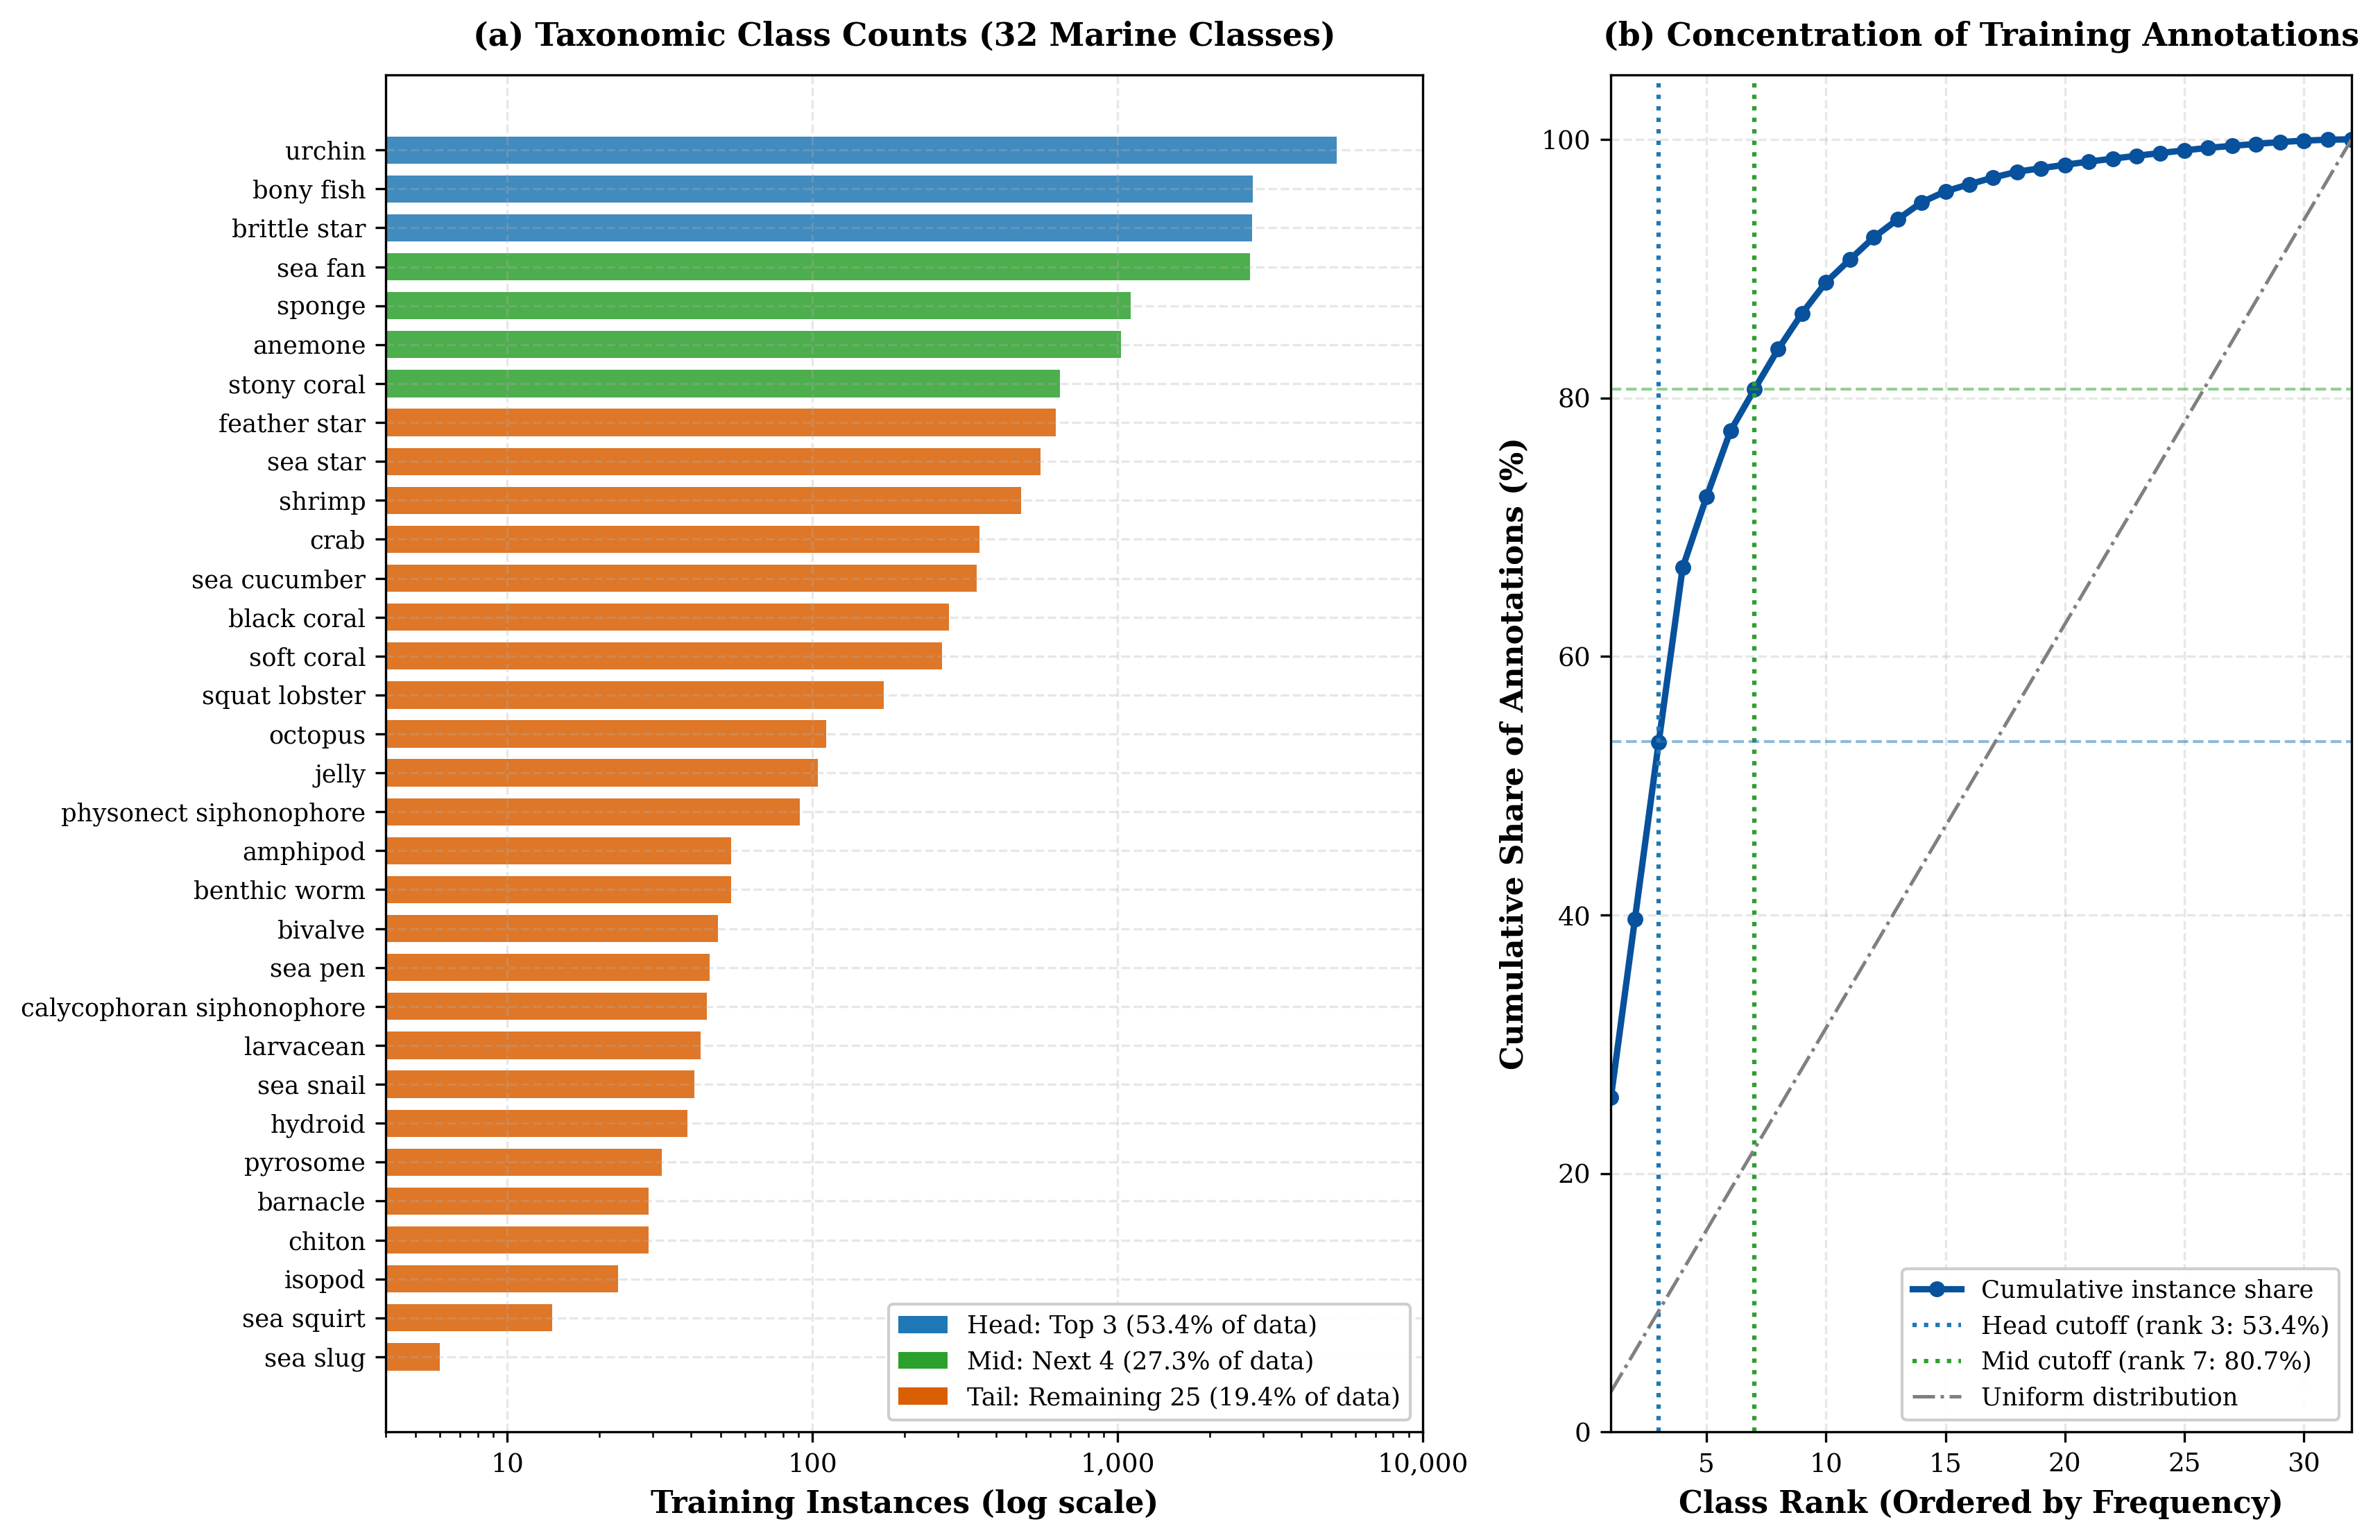
\includegraphics[width=0.92\textwidth]{images/fig_class_imbalance.png}
  \caption{Taxonomic class distribution and annotation concentration across the 32 FathomNet CLEF~2026 categories. (a)~Training instance counts per class on a logarithmic scale, highlighting the three frequency strata: Head (blue, top 3 classes, 53.4\% of annotations), Mid (green, next 4 classes, 27.3\%), and Tail (orange, remaining 25 classes, 19.4\%). (b)~Cumulative annotation share demonstrating extreme Pareto inequality, where the top 7 taxa account for over 80\% of all instances.}
  \label{fig:class-imbalance}
\end{figure*}

\begin{table}[t]
  \centering
  \small
  \caption{Per-class instance counts (train and validation) and the
  head/mid/tail stratification across the 32 marine categories. Classes are ordered by decreasing training-instance count.}
  \label{tab:class-counts}
  \setlength{\tabcolsep}{3pt}
  \begin{tabular}{llrr}
    \toprule
    Stratum & Class & Train & Val \\
    \midrule
    head & urchin & 5{,}212 & 511 \\
    head & bony fish & 2{,}768 & 301 \\
    head & brittle star & 2{,}761 & 252 \\
    mid  & sea fan & 2{,}715 & 311 \\
    mid  & sponge & 1{,}101 & 112 \\
    mid  & anemone & 1{,}026 & 98 \\
    mid  & stony coral & 646 & 95 \\
    tail & feather star & 628 & 59 \\
    tail & sea star & 558 & 66 \\
    tail & shrimp & 483 & 42 \\
    tail & crab & 353 & 42 \\
    tail & sea cucumber & 346 & 32 \\
    tail & black coral & 280 & 44 \\
    tail & soft coral & 265 & 27 \\
    tail & squat lobster & 171 & 18 \\
    tail & octopus & 111 & 11 \\
    tail & jelly & 104 & 10 \\
    tail & physonect siphonophore & 91 & 10 \\
    tail & amphipod & 54 & 4 \\
    tail & benthic worm & 54 & 6 \\
    tail & bivalve & 49 & 7 \\
    tail & sea pen & 46 & 4 \\
    tail & calycophoran siphonophore & 45 & 1 \\
    tail & larvacean & 43 & 4 \\
    tail & sea snail & 41 & 11 \\
    tail & hydroid & 39 & 2 \\
    tail & pyrosome & 32 & 4 \\
    tail & barnacle & 29 & 2 \\
    tail & chiton & 29 & 7 \\
    tail & isopod & 23 & 5 \\
    tail & sea squirt & 14 & 3 \\
    tail & sea slug & 6 & 1 \\
    \bottomrule
  \end{tabular}
\end{table}

\subsection{Image and object geometry}
\label{sec:data-geometry}

The competition imagery is full-resolution JPEG, with frame sizes varying
widely across source vehicles and cruises; no resizing or tiling is applied
before training, and each detector instead applies its native input policy
(\S\ref{sec:methods-frcnn}--\S\ref{sec:methods-rtdetr-l}): Faster R-CNN
resize to a nominal square 640\,px input (framework-side resizing rules still differ).
A systematic audit of frame resolutions, bounding-box scales under standard COCO conventions, and aspect-ratio distributions confirms that 100\% of images are widescreen 16:9 frames (split evenly between 1080p Full HD and 4K Ultra HD), while small objects ($<32$\,px) represent fewer than 0.5\% of annotated instances (detailed in Figure~\ref{fig:eda-geometry} in Appendix~\ref{app:eda}).

\subsection{Split protocol}
\label{sec:data-split}

All models in this paper are trained and evaluated on a single stratified
90/10 image-level split initialized with random seed~42. Stratification is
enforced at the image level to ensure that no image appears in both partitions,
yielding $5{,}817$ training images and $646$ validation images containing
$2{,}102$ annotated instances across all $32$ taxonomic classes. The split is
frozen across all experiments so that all three detectors are trained and scored
on an identical dataset partition; the held-out test set remains untouched.

\section{Methods}
\label{sec:methods}

This section describes the detectors, the shared evaluation protocol, and the
training setup used throughout the study. Three detectors are benchmarked ---
the two-stage Faster R-CNN R50-FPN~\cite{fasterrcnn2015}, the one-stage
YOLOv8s~\cite{yolov8_2023}, and the transformer-based RT-DETR-L~\cite{rtdetr2024}
--- covering the three dominant architectural families. All three runs have
completed, and every number reported in this paper comes from a finished
training run. An RT-DETR-R18 variant was originally planned as a fourth
detector to probe the effect of scaling within the RT-DETR family, but it was
dropped for compute-budget reasons and is not reported here. Each detector was trained within a standardized execution environment
using the frozen stratified split and evaluated using a common COCO
bounding-box evaluation protocol implemented via \texttt{pycocotools}~\cite{pycocotools}.

\subsection{Evaluation protocol}
\label{sec:eval}

All detectors are evaluated with the same COCO-style bounding-box protocol
implemented as a unified, shared evaluation harness. The evaluation
closely follows the standard \texttt{pycocotools} recipe~\cite{coco2014}
and produces three families of numbers: the overall mAP averaged over IoU
thresholds, the per-class AP, and the head/mid/tail stratum aggregates used as
the paper's primary summary statistics.

\textbf{Ground truth.} Ground-truth annotations for the validation set are constructed
directly from the official FathomNet development annotations corresponding to the
frozen validation partition ($646$ images and $2{,}102$ annotations across all
$32$ taxonomic categories). The identical ground-truth set is loaded with
\texttt{coco.COCO} for every model, ensuring that all evaluation is performed against
identical reference annotations.

\textbf{Detection format.} Each model's predictions are formatted as standard
COCO detection records
\{\texttt{image\_id}, \texttt{category\_id}, \texttt{bbox} $[x,y,w,h]$,
\texttt{score}\}, where the category id matches the original FathomNet category indexing.
For the TorchVision model the raw network outputs (boxes in
$[x_1,y_1,x_2,y_2]$, labels in \texttt{category\_id\,+\,1} form) are converted
back to this format; for the two Ultralytics models the native predictions
are mapped directly to the same COCO representation. All predictions are preserved
in structured format so evaluation can be reproduced without re-inference.

\textbf{score threshold and detection cap.} Detections are filtered to those with
a confidence score above $0.001$, and at most $300$ detections per image are kept
(after thresholding, sorted by score). These are the same thresholds used in the
evaluation harness and are computed identically across all three models.

\textbf{Metrics.} For each model \texttt{coco\_eval()} runs
\texttt{COCOeval.evaluate()}, \texttt{.accumulate()}, and \texttt{.summarize()}
once over the full validation set to obtain the two summary statistics reported in
the main results table:
\begin{itemize}
  \item \textbf{mAP50-95} --- the COCO primary metric, the mean average precision
        averaged over $10$ IoU thresholds from $0.50$ to $0.95$ in steps of $0.05$
        (the \texttt{E.stats[0]} value in \texttt{pycocotools});
  \item \textbf{mAP50} --- the average precision at IoU threshold $0.50$
        (\texttt{E.stats[1]}).
\end{itemize}
Per-class AP is then obtained by repeating the evaluate/accumulate/summarize cycle
once per category, restricting \texttt{COCOeval.params.catIds} to a single class
each time, and recording \texttt{E.stats[0]} (the AP at the full IoU sweep) for
that class. This produces a \texttt{per\_class\_AP50-95} dictionary with one entry
per FathomNet category; it is the source for both the full per-class table in
Appendix~\ref{app:perclass} and the stratum aggregates below.

\textbf{Head/mid/tail aggregation.} Per-class AP values are aggregated into the
three strata defined in Section~\ref{sec:data-imbalance} by taking the unweighted
mean of the per-class AP within each stratum:
\[
\mathrm{AP}_{\mathrm{stratum}} = \frac{1}{|\mathcal{C}_{\mathrm{stratum}}|}
\sum_{c \in \mathcal{C}_{\mathrm{stratum}}} \mathrm{AP}(c).
\]
The strata are fixed from the training label counts (3 / 4 / 25 classes,
head/mid/tail) and are identical across all models. The aggregation computes unweighted stratum means and feeds the
head/mid/tail columns of Table~\ref{tab:main}. This aggregation is the paper's
primary way of summarising long-tail behaviour because per-class AP on the 25 tail
classes is noisy (several tail classes have only a handful of validation instances,
as discussed in Section~\ref{sec:data-imbalance}); the stratum means smooth out
that noise while still exposing the head-to-tail degradation that is the central
question of the benchmark.

\textbf{Latency.} Inference latency is reported as the median wall-clock time of
$30$ single-image forward passes, after $5$ warm-up passes, measured on the same
validation image for every model. For the TorchVision models the measurement
brackets a forward pass of a synthetic $800\times1280$ tensor with explicit
CUDA synchronisation before and after; for the Ultralytics models it brackets a
call to \texttt{best.predict()} on a single real validation image loaded with
OpenCV. The latency figures are reported per image in milliseconds and reflect the
models' nominal 640\,px input size (framework-side resizing rules still differ).


\subsection{Faster R-CNN R50-FPN}
\label{sec:methods-frcnn}

Faster R-CNN~\cite{fasterrcnn2015} is the two-stage, anchor-based detector in the
benchmark. It is implemented in \texttt{torchvision} and initialised from
COCO-pretrained weights (\texttt{weights='COCO\_V1'}). The backbone is a ResNet-50 with
a Feature Pyramid Network (FPN) that builds a multi-scale feature representation from
the final convolution outputs of the ResNet stages. In the first stage, a region proposal
network (RPN) takes the FPN features and predicts a set of region proposals (anchors at
multiple scales and aspect ratios) with objectness scores. In the second stage, the
proposed regions are pooled to a fixed size with RoIAlign and passed to a box head that
predicts per-region class scores and bounding-box refinements. The box predictor head is
replaced with a \texttt{FastRCNNPredictor(1024, n\_cls)} so that the model can output
scores for the $32$ FathomNet classes (plus background).

We implement Faster R-CNN using PyTorch and TorchVision. The dataset is configured with a
custom \texttt{torch.utils.data.Dataset} that loads each image from disk, converts it to an
RGB tensor, and builds a target dict with \texttt{boxes} in $[x_1,y_1,x_2,y_2]$ form,
\texttt{labels} as \texttt{category\_id$+$1} (with $0$ reserved for background), area, and
image id. The only augmentation is a random horizontal flip applied with probability $0.5$
during training, with the box coordinates updated accordingly; no cropping, scaling, or
colour augmentation is used. The model is trained for \emph{30 epochs} with stochastic gradient descent (learning rate $0.0025$, momentum $0.9$, weight decay $1\times 10^{-4}$), a step scheduler that halves the learning rate after the final epoch, and gradient clipping to a maximum norm of $10.0$. The training batch size is $2$ images per step (the native TorchVision two-stage model does not batch in the same way as one-stage detectors, and the small batch reflects GPU memory on the Kaggle T4), with $2$ prefetch workers and pinned memory; the validation loader uses batch size $4$. The nominal input size is $640$\,px. The run is a \emph{resumed} 30-epoch run: training resumes from a previously saved checkpoint (resuming from a pre-trained intermediate checkpoint) and continues to epoch~30 on the same split, so all three detectors share the same nominal epoch budget even though framework resizing, optimisers, augmentation, and checkpoint-selection rules still differ (see \S\ref{sec:methods-training}).

At inference the model runs in evaluation mode on the validation set; for each image the predicted boxes, scores, and labels are thresholded at a score of $0.001$, truncated to at most $300$ detections, converted from $[x_1,y_1,x_2,y_2]$ to $[x,y,w,h]$ form, and written to a COCO-format JSON as predictions. The network outputs category labels offset by one (because of the background class), so the \texttt{category\_id} is recovered by subtracting one before writing. Inference latency is reported as the median wall-clock time over $30$ single-image forward passes at the nominal $640$\,px input size (batch~1, FP32, decoded RGB to CPU detections, excluding disk/decode), after $5$ warm-up passes, with explicit CUDA synchronisation before and after each timed pass. The number of trainable parameters is computed dynamically from the model after the head replacement.

\subsection{YOLOv8s}
\label{sec:methods-yolov8s}

YOLOv8s~\cite{yolov8_2023} is the one-stage, anchor-free detector in the
benchmark, implemented in the Ultralytics framework and initialised from a
COCO-pretrained checkpoint. The architecture follows the YOLOv8 design: a
CSPDarknet-style backbone with C2f blocks, a path-aggregation neck, and a
decoupled head that separates classification from box regression, with box
targets represented as a discrete distribution over offsets rather than a
single point estimate. Detections are produced directly on the output grid
and refined by a distribution-focal-loss---driven regression, with NMS at
inference; training uses the built-in Ultralytics augmentation pipeline
(mosaic, random scale/translate/flip, HSV jitter, and mixup) with the
default close-mosaic schedule.

We train YOLOv8s within the Ultralytics framework. A
YOLO-format dataset is configured from the shared split: the original FathomNet
category ids are remapped to a contiguous $0$--$31$ range, one normalised
label file is written per image, and images are symlinked to avoid copying.
The model is trained for 30 epochs with \texttt{imgsz}$\,{=}\,640$ (the nominal input size shared by all three runs), a batch size of~$4$ per GPU forward pass, one data worker, and disk caching of decoded images --- a configuration chosen to keep peak GPU memory within a single T4. The optimiser is selected automatically by Ultralytics
(\texttt{optimizer=auto}), resolving to AdamW with lr
$2.78\times10^{-4}$ and momentum $0.9$, with \texttt{amp=True} for mixed
precision and early stopping configured with a patience of~50 epochs. No
other hyperparameters are modified from their defaults.

At inference the best checkpoint (highest validation fitness over the 30 epochs) is loaded and run on the validation images with \texttt{conf}$\,{=}\,0.001$, \texttt{iou}$\,{=}\,0.7$, \texttt{max\_det}$\,{=}\,300$, and \texttt{imgsz}$\,{=}\,640$. Predictions are mapped back to the original category ids and written to a COCO-format JSON for the shared evaluation, and inference latency is measured as the median wall-clock time of 30 single-image forward passes at the nominal $640$\,px input size (batch~1, FP32) after five warm-up passes.

\subsection{RT-DETR}
\label{sec:methods-rtdetr-r18}

RT-DETR~\cite{rtdetr2024} is the transformer-based, end-to-end detector in the benchmark.
It is implemented in the Ultralytics framework and initialised from a COCO-pretrained
checkpoint. The architecture follows the RT-DETR design: a ResNet backbone produces a
multi-scale feature pyramid, which is fed into an efficient hybrid encoder that
reformulates the multi-scale features into image features suitable for attention-based
processing, and a transformer decoder that directly predicts a fixed set of object
queries. Unlike the Faster R-CNN and YOLOv8s pipelines, RT-DETR is end-to-end: it
predicts the full set of detections in a single forward pass without requiring a
non-maximum suppression (NMS) post-processing step. The decoder uses auxiliary
prediction heads during training to stabilise learning, and the model is trained with a
convex combination of classification, regression, and auxiliary losses.

An RT-DETR-R18 variant was originally planned so that the transformer architecture
could be compared across two backbone scales, but only the large variant
(\S\ref{sec:methods-rtdetr-l}) was trained within the available compute budget;
all RT-DETR results in this paper refer to the large variant.

\subsection{RT-DETR-L}
\label{sec:methods-rtdetr-l}

RT-DETR-L~\cite{rtdetr2024} is the large variant of the same RT-DETR family and is included
as the larger-scale representative of the transformer-based detector. The architecture is
the same end-to-end RT-DETR design described in \S\ref{sec:methods-rtdetr-r18}: a ResNet backbone,
an efficient hybrid encoder, and a transformer decoder that predicts a fixed set of object
queries without NMS post-processing. The ``$L$'' variant uses a larger backbone than
the RT-DETR base configuration and therefore a larger feature extractor and a higher-capacity decoder; it is
included so that the effect of scaling the RT-DETR architecture can be observed within the
same benchmark, and to test whether the larger model overcomes the long-tail degradation
observed for the other detectors.

We train RT-DETR-L within the Ultralytics environment. The same
YOLO-format dataset conversion used for YOLOv8s is applied: the original
category ids are remapped to a contiguous $0$--$31$ range, one normalised label file is
written per image, and images are symlinked to avoid copying. The model is trained for 30
epochs with \texttt{imgsz}$\,{=}\,640$ (the default input size), a batch size of~$4$ per GPU
forward pass, one data worker, disk caching of decoded images, and \texttt{amp}$\,{=}\,$
\texttt{True} (automatic mixed precision) enabled. The larger backbone makes this variant the
most memory-demanding of the three detectors; the batch size and the mixed-precision setting
are both chosen to keep the peak GPU memory within the capacity of a single T4 GPU. The batch size and mixed-precision settings are specifically tailored to maintain peak memory usage within 15\,GiB. The default Ultralytics optimiser and the built-in training augmentations are
used without modification. Early stopping is configured with a patience of~50 epochs.

At inference the best checkpoint is loaded and run on the validation images with
\texttt{conf}$\,{=}\,0.001$, \texttt{iou}$\,{=}\,0.7$, \texttt{max\_det}$\,{=}\,300$, and
\texttt{imgsz}$\,{=}\,640$. As with every RT-DETR configuration, the raw decoder outputs are used directly
as the detections, with no NMS applied, and predictions are mapped back to the original
category ids and written to a COCO-format JSON for evaluation. Inference latency is measured
as the median wall-clock time of $30$~single-image forward passes at the native input size,
after five warm-up passes. Inference latency for all three runs is reported in Table~\ref{tab:main} and \S\ref{sec:results-latency}.

\subsection{Common training details}
\label{sec:methods-training}

All three models share the same data, split, and evaluation code path. All models
share identical training and validation splits initialized with random seed~42;
the validation partition is frozen across models, so all reported differences are
attributable to the detector, not the data. Training was executed on
remote single-GPU instances (NVIDIA T4, 15\,GiB); both Ultralytics models
were trained with \texttt{amp=True} (automatic mixed precision), batch
size~4, and a single data worker with disk caching of decoded images, which
keeps the peak memory within the T4 capacity. The Faster R-CNN run used
single precision. Hyperparameters were selected by the authors rather than
tuned per model --- all three runs use a nominal 30 epochs at 640\,px, but framework resizing, optimisers, and checkpoint-selection rules differ --- so comparisons across families
should be read as representative of default configurations rather than
tuned optima; this is restated as a limitation in
\S\ref{sec:limitations}. Framework versions (TorchVision for Faster R-CNN; Ultralytics for YOLOv8s
and RT-DETR-L) are pinned in the project environment.

\section{Results}
\label{sec:results}

All numbers in this section are computed on the local stratified validation
split ($646$ images, $2{,}102$ instances) with the shared COCO-style
protocol of \S\ref{sec:eval}. All three training runs have completed; no
number in this paper is a projection or a partial result. Where the
Ultralytics internal validation loop and the COCO re-evaluation differ
slightly (the internal loop uses its own IoU smoothing and class-weighting),
this paper always reports the COCO re-evaluation numbers, which are the
values produced by the shared COCO evaluation tool.

\begin{table*}[t]
  \centering
  \small
  \caption{Detector benchmark on FathomNet CLEF~2026 under an identical
  stratified validation split and a single COCO-style evaluation protocol.
  mAP values are averaged over IoU thresholds 0.50--0.95. Head, mid, and tail
  are per-class AP averaged over the strata defined in
  \S\ref{sec:data-imbalance}. Latency is the median wall-clock time of $30$
  single-image forward passes on the training GPU (T4), excluding
  pre- and post-processing unless noted; per-image inference speed is
  reported separately in \S\ref{sec:results-latency}. All values come from the completed benchmark runs on the frozen validation partition.}
  \label{tab:main}
  \setlength{\tabcolsep}{4pt}    % default is 6pt
  \begin{tabular*}{0.9\textwidth}{@{\extracolsep{\fill}}L{3.4cm}rrrrrrr@{}}
    \toprule
    Detector & Params (M) & mAP & mAP$_{50}$ & Head & Mid & Tail & Latency (ms) \\
    \midrule
    Faster R-CNN R50-FPN & 41.3 & 0.333 & 0.483 & 0.451 & 0.424 & 0.305 & 46.4 \\
    YOLOv8s              & 11.1 & 0.313 & 0.428 & 0.436 & 0.408 & 0.283 & 24.0  \\
    RT-DETR-L            & 32.9 & 0.231 & 0.323 & 0.429 & 0.345 & 0.189 & 62.2  \\
    \bottomrule
  \end{tabular*}
\end{table*}

\begin{figure*}[t]
  \centering
  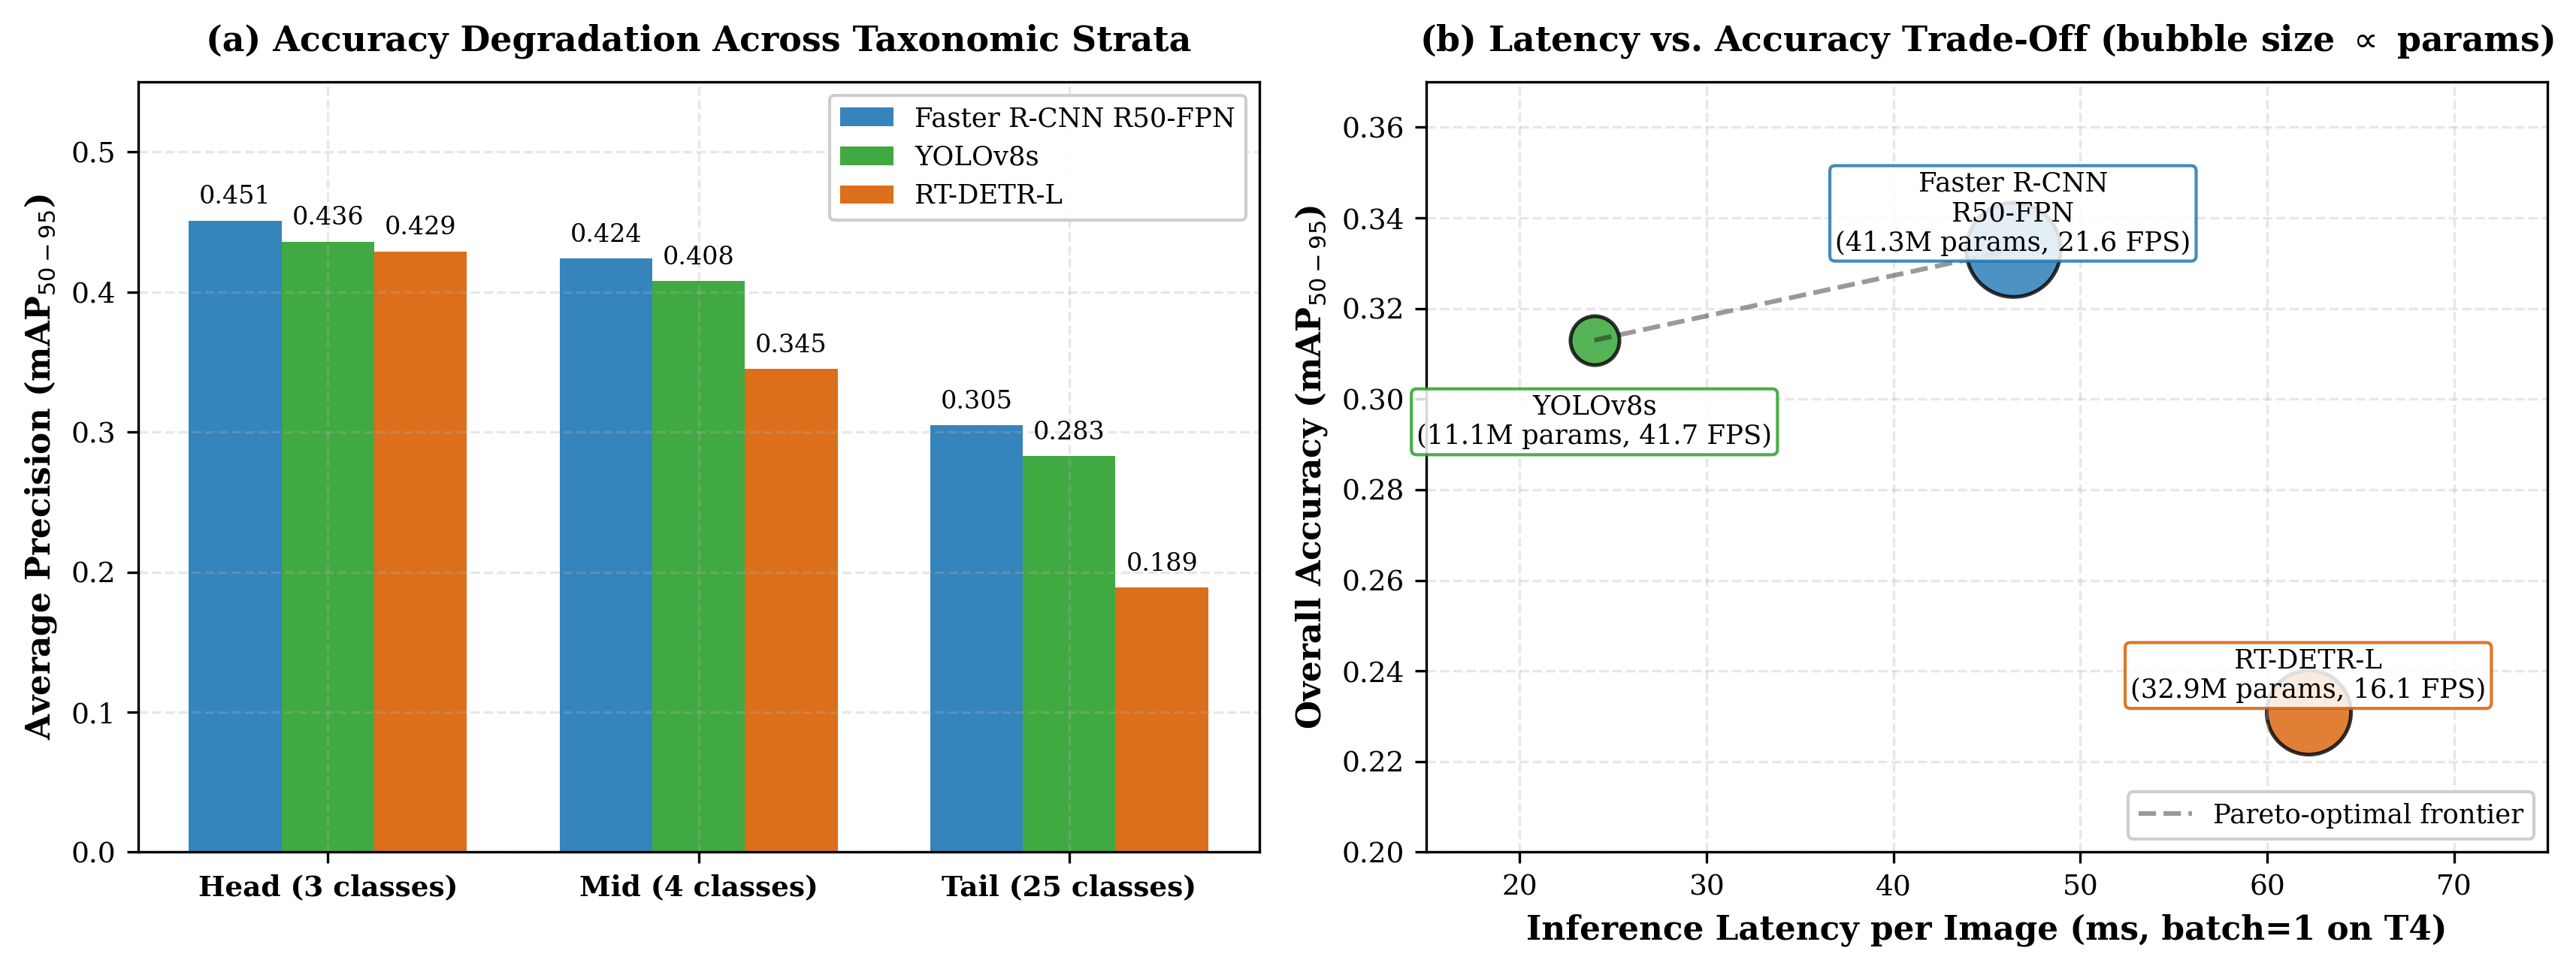
\includegraphics[width=0.92\textwidth]{images/fig_performance_tradeoff.png}
  \caption{Detector benchmark analysis on FathomNet CLEF~2026. (a)~Accuracy degradation across taxonomic frequency strata (Head, Mid, Tail), demonstrating consistent performance loss across all three architectures, with Faster R-CNN exhibiting the highest tail retention. (b)~Inference latency versus overall mAP$_{50\text{-}95}$ trade-off on an NVIDIA T4 GPU (FP32, batch~1); bubble area is proportional to parameter count (11.1M for YOLOv8s, 32.9M for RT-DETR-L, 41.3M for Faster R-CNN). The dashed line denotes the empirical Pareto-optimal frontier.}
  \label{fig:performance-tradeoff}
\end{figure*}



\subsection{Main comparison}
\label{sec:results-main}

The ranking in Table~\ref{tab:main} is unambiguous under the nominally equal 30-epoch, 640\,px setup: Faster R-CNN R50-FPN leads on every aggregate, with mAP$_{50\text{-}95}=0.333$ and mAP$_{50}=0.483$; YOLOv8s follows at $0.313/0.428$; and RT-DETR-L trails at $0.231/0.323$. The margin between the leading and trailing detectors is $+0.102$~mAP$_{50\text{-}95}$ from Faster R-CNN to RT-DETR-L. Because framework resizing, optimisers, and checkpoint-selection rules differ, this ordering compares representative default training setups rather than equal compute, and it should not be read as a general law about detector families.

The per-epoch training curves in Figure~\ref{fig:training-curves} show the three runs side by side on the shared validation split. All three use the same confidence threshold ($0.001$) and detection cap ($300$); the remaining differences (resizing rules, optimisers, augmentation, checkpoint selection) are documented in \S\ref{sec:methods-training} and Appendix~\ref{app:hyperparams}. Notably, RT-DETR-L emits the full 300 detections per image on average (score mean $0.061$) while Faster R-CNN emits far fewer ($18.9$ per image, score mean $0.178$), so the shared threshold does not imply equally selective prediction sets.

On speed--accuracy balance, Faster R-CNN leads on accuracy here while YOLOv8s is the fastest ($24.0$\,ms versus $46.4$\,ms for Faster R-CNN and $62.2$\,ms for RT-DETR-L at batch~1, FP32, on a T4). The implications for on-platform deployment are discussed in \S\ref{sec:results-latency}.

\begin{figure*}[t]
  \centering
  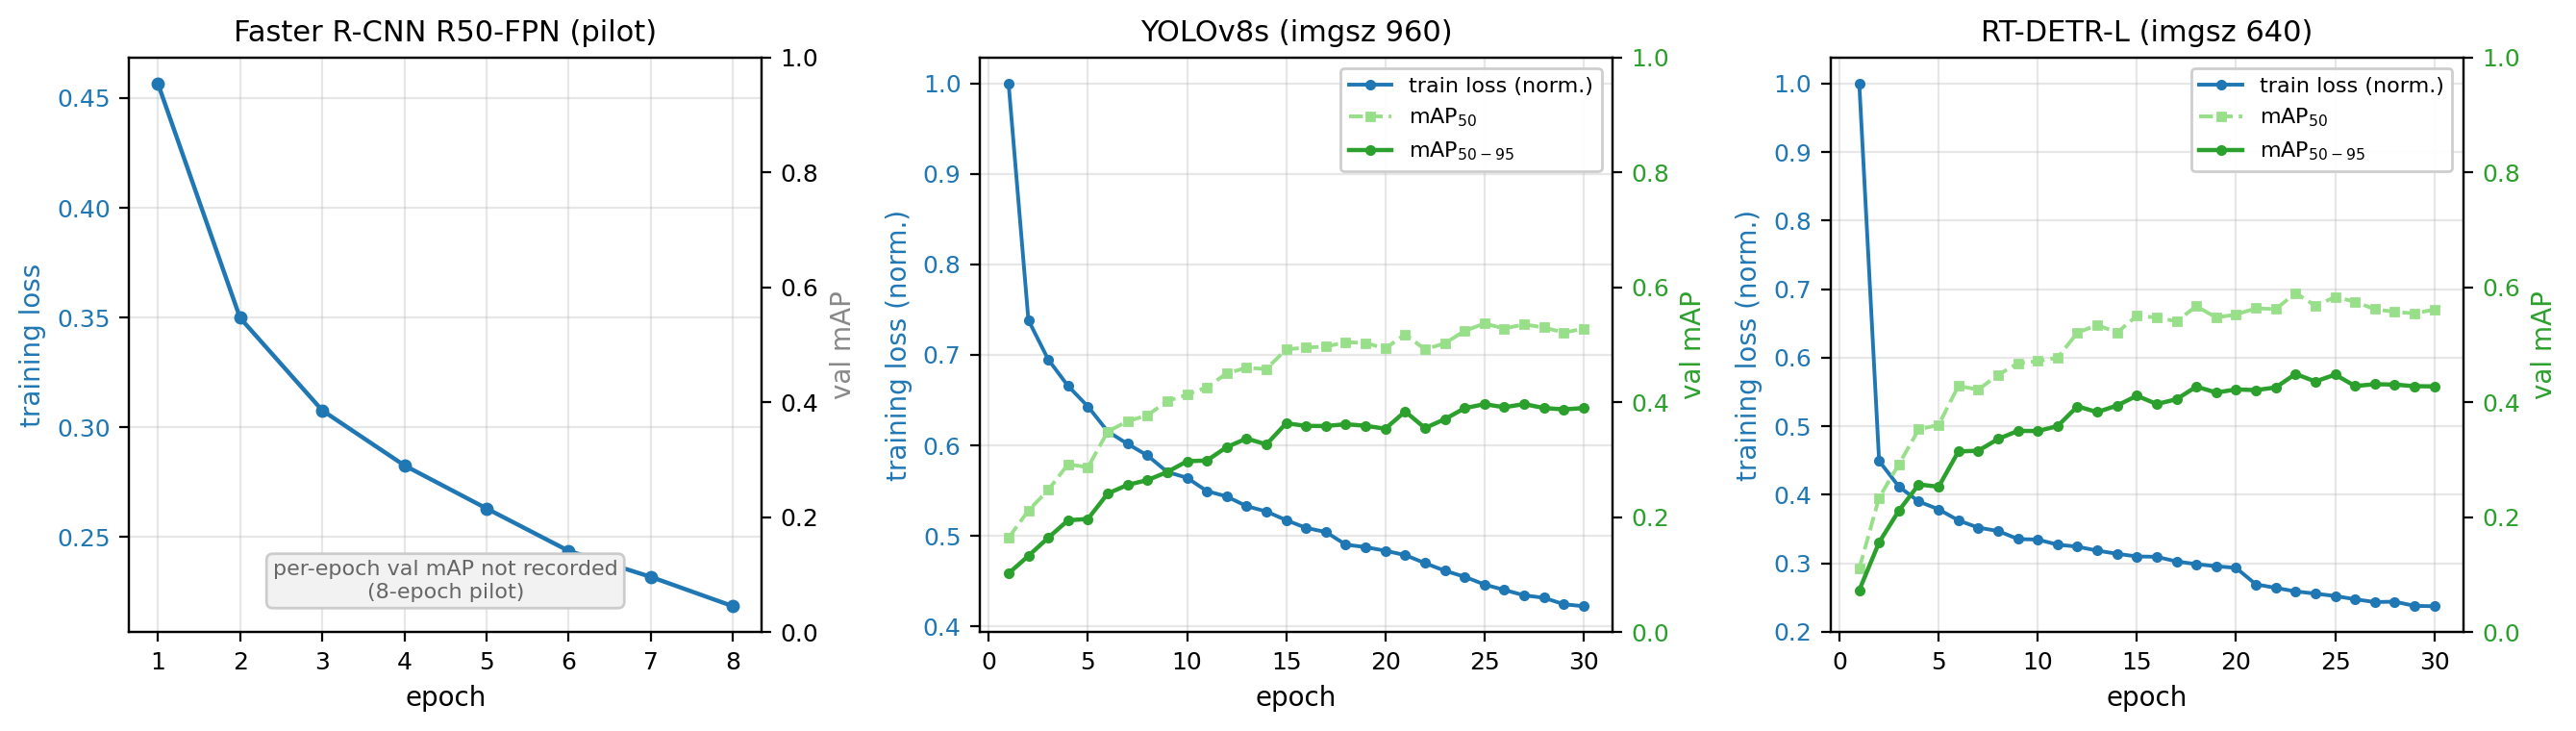
\includegraphics[width=\textwidth]{images/curve_all.png}
  \caption{Training and validation curves for the three completed runs,
  all on the shared validation split. Blue (left axis): total training
  loss per epoch (sum of loss components; normalised to the epoch-1
  value for the two Ultralytics models). Green (right axis): validation
  mAP$_{50}$ and mAP$_{50\text{-}95}$. (Left) Faster R-CNN R50-FPN, 30 epochs (resumed run) at nominal 640\,px. (Center) YOLOv8s, 30 epochs at nominal 640\,px. (Right) RT-DETR-L, 30 epochs at nominal 640\,px. Curves share the validation split but reflect each framework's own loss and validation definitions, so only within-panel trends should be compared.}
  \label{fig:training-curves}
\end{figure*}

\subsection{Per-class analysis}
\label{sec:results-perclass}

The per-class AP tables for all three detectors are given in Appendix~\ref{app:perclass}. A consistent pattern emerges: the classes that are hard for one architecture are hard for all of them. The five classes with zero or near-zero AP across the board --- \textit{sea slug} (1 validation instance), \textit{sea squirt} (3), \textit{amphipod} (4), \textit{benthic worm} (6), and \textit{bivalve} (7) --- are precisely the rarest classes, and none of the three detectors learns a usable detector for them from so few examples. At the other end, the same taxa are easy for every architecture: \textit{pyrosome} (AP$_{50\text{-}95}$ $0.888$--$0.925$ across the three runs), \textit{larvacean} ($0.595$--$0.718$), \textit{soft coral} ($0.542$--$0.578$), \textit{crab} ($0.517$--$0.594$), \textit{urchin} ($0.516$--$0.592$), and \textit{stony coral} ($0.429$--$0.586$) combine high distinctiveness with moderate-to-large instance counts.

Morphology explains much of the per-class structure. Soft-bodied, translucent taxa with variable silhouette (\textit{jelly}, \textit{larvacean}, \textit{salp-like siphonophores}) yield mid-range AP despite few instances, whereas cryptic, substrate-mimicking taxa (\textit{squat lobster}, \textit{shrimp}) sit in the middle-to-low range even with dozens of instances. No detector dominates every tail class: Faster R-CNN leads on \textit{hydroid} ($0.654$ versus $0.455$ for YOLOv8s and $0.000$ for RT-DETR-L), \textit{larvacean} ($0.718$ versus $0.628$ and $0.595$), and \textit{barnacle} ($0.454$ versus $0.404$ and $0.000$), while YOLOv8s leads on \textit{chiton} ($0.601$ versus $0.443$ and $0.506$) and \textit{sea pen} ($0.410$ versus $0.222$ and $0.000$).

\subsection{Head, mid, and tail degradation}
\label{sec:results-headmidtail}

Head/mid/tail degradation is large and directional for every architecture (Table~\ref{tab:main} and Figure~\ref{fig:performance-tradeoff}a). Faster R-CNN drops $0.146$~AP$_{50\text{-}95}$ from head ($0.451$) to tail ($0.305$) --- a $32\%$ relative drop; YOLOv8s drops $0.153$ ($0.436 \to 0.283$, $35\%$ relative); RT-DETR-L drops $0.240$ ($0.429 \to 0.189$, $56\%$ relative). Two observations matter. First, the stratum ordering (head $>$ mid $>$ tail) is identical for all three families, confirming that the long tail is a property of the task, not of any particular detector. Second, the \emph{size} of the tail penalty differs: here the two-stage detector degrades the least and the transformer degrades the most, but because optimisers, augmentation, and checkpoint selection differ across frameworks this should not be read as a general family-level law. Long-tail-aware training (class-balanced sampling, focal-loss re-weighting, or copy-paste augmentation for the tail) is the natural next step and is discussed in \S\ref{sec:discussion}.

\subsection{Object-size sensitivity}
\label{sec:results-size}

The object-size breakdown (COCO small/medium/large buckets, Table~\ref{tab:size}) shows the same ordering at every scale: Faster R-CNN leads on large objects ($0.377$) ahead of YOLOv8s ($0.350$) and RT-DETR-L ($0.254$), and the gap widens on medium objects where RT-DETR-L ($0.075$) is closest to YOLOv8s ($0.063$) and Faster R-CNN ($0.059$). Small objects are effectively undetected by all three runs (AP $0.007$ for Faster R-CNN, $0.000$ for both Ultralytics runs), consistent with the $640$\,px nominal input and the rarity of small annotated instances in the validation split.

\begin{table}[t]
  \centering
  \small
  \caption{COCO size-stratified AP$_{50\text{-}95}$ (small/medium/large)
  from the shared re-evaluation. Small objects are effectively
  undetected at the nominal 640\,px input.}
  \label{tab:size}
  \setlength{\tabcolsep}{2pt}
  \begin{tabular*}{\columnwidth}{@{\extracolsep{\fill}}lccc@{}}
    \toprule
    Detector & Small & Medium & Large \\
    \midrule
    Faster R-CNN R50-FPN & 0.007 & 0.059 & 0.377 \\
    YOLOv8s & 0.000 & 0.063 & 0.350 \\
    RT-DETR-L & 0.000 & 0.075 & 0.254 \\
    \bottomrule
  \end{tabular*}
\end{table}

\subsection{Inference cost}
\label{sec:results-latency}

Latency was measured on the training hardware (NVIDIA T4) as the median wall-clock time of 30 single-image forward passes at the nominal 640\,px input size, after five warm-up passes (Table~\ref{tab:main}; batch~1, FP32, decoded RGB to CPU detections, excluding disk/decode; see \S\ref{sec:eval}). YOLOv8s is the fastest detector at $24.0$\,ms per image, Faster R-CNN R50-FPN intermediate at $46.4$\,ms, and RT-DETR-L slowest at $62.2$\,ms.

For on-platform deployment the trade-off is clear (Figure~\ref{fig:performance-tradeoff}b). Faster R-CNN is the accuracy leader here but costs $1.9\times$ the latency of YOLOv8s; YOLOv8s reaches $94\%$ of Faster R-CNN's mAP$_{50\text{-}95}$ ($0.313$ versus $0.333$) at $52\%$ of its latency and with roughly a quarter of its parameters, and it fits comfortably on a 15\,GiB GPU with room for the rest of a vehicle's software stack. RT-DETR-L is neither the most accurate nor the fastest in this configuration, so it is best viewed as the transformer-family baseline rather than a deployment recommendation from these runs.

\subsection{Qualitative examples}
\label{sec:results-qualitative}

Figure~\ref{fig:qualitative} (Appendix~\ref{app:eda}) presents matched qualitative detection panels across architectures on representative validation frames at a score threshold of $0.25$, with ground-truth bounding boxes overlaid. Figure~\ref{fig:gradcam} presents high-resolution Grad-CAM visual attributions on the same scenes, comparing feature activation patterns across deep network layers. The panels illustrate the per-class findings above (\S\ref{sec:results-perclass}) rather than isolated anecdotes --- in particular, side-by-side frames from the easiest (\textit{urchin}, \textit{pyrosome}) and hardest (\textit{sea slug}, \textit{amphipod}) classes.

\section{Discussion}
\label{sec:discussion}

The ranking --- two-stage $>$ one-stage $>$ transformer in this nominally equal 30-epoch, 640\,px configuration --- must be read with the configuration caveat in \S\ref{sec:methods-training} rather than as a law about detector families. All three runs share the split, confidence threshold, detection cap, and nominal epoch/resolution budget, but framework resizing, optimisers, augmentation, and checkpoint-selection rules differ, so these numbers compare representative default training setups. The head/mid/tail degradation shared by all three runs is nevertheless inherited directly from the data distribution, and the per-class pattern (\S\ref{sec:results-perclass}) is consistent across families.

The memory footprint also has a practical implication. Both Ultralytics runs used mixed precision (\texttt{amp=True}) with batch~4 to fit on a 15\,GiB T4, while the Faster R-CNN run used batch~2 in single precision;
substantially larger batch sizes or higher input resolutions would
require more memory than a single commodity GPU provides. For a
benchmark of this size, YOLOv8s sits at the sweet spot of the
accuracy--cost curve, and Faster R-CNN is the accuracy ceiling in this configuration.

Which findings are likely to transfer? The head-to-tail degradation
ordering should generalise to any long-tailed underwater dataset, since
it follows directly from instance counts; the family ranking is confounded by framework resizing, optimisers, augmentation, and checkpoint-selection differences, and should be re-checked on other benchmarks before being treated as a law. The per-class failures on near-zero-instance classes
are certainly dataset-specific but illustrate a general point: no
detector family recovers a class from six training examples without
long-tail-specific interventions.

Long-tail-aware training is the obvious next step for this benchmark:
class-balanced sampling or loss re-weighting for the 25 tail classes,
copy-paste augmentation for the five classes with fewer than ten
validation instances, and possibly a two-stage fine-tune on the tail.
Given that the stratum gap costs $0.146$--$0.240$~AP depending on the run, closing even a third of it would move the overall benchmark numbers materially.

\section{Limitations}
\label{sec:limitations}

This study has several limitations. All three runs use a nominal 30 epochs at 640\,px, but framework resizing, optimisers, augmentation, and checkpoint-selection rules differ (see \S\ref{sec:methods-training} and Appendix~\ref{app:hyperparams}), so the nominal budget is not equal compute and the ranking should be treated as indicative rather than definitive. All results are on a
single validation split with a single random seed, so no variance
estimate is reported; and the blind test set is untouched, so no
leaderboard comparison is possible yet. Latency was measured on one hardware platform (T4) at one batch size; the qualitative panels reflect the fixed validation-image selection (seed~42) rather than success-filtered examples. Finally, the
planned RT-DETR-R18 scale comparison was dropped for compute-budget
reasons, so within-family scaling of the RT-DETR architecture is not
evaluated.

\section{Conclusion}
\label{sec:conclusion}

This paper benchmarked three object detectors --- Faster R-CNN R50-FPN,
YOLOv8s, and RT-DETR-L --- on FathomNet CLEF~2026 under a single
stratified split (seed~42) and a shared COCO-style evaluation protocol
with identical confidence and detection-cap settings. Every reported
metric is derived from a verified training and evaluation run under an
open experimental protocol.

Three findings stand out. First, Faster R-CNN is the strongest detector on every aggregate in this nominally equal 30-epoch, 640\,px configuration (mAP$_{50\text{-}95}=0.333$, mAP$_{50}=0.483$), ahead of YOLOv8s ($0.313/0.428$) and RT-DETR-L ($0.231/0.323$), with the framework-difference caveat of \S\ref{sec:methods-training}. Second, the long tail dominates the difficulty: every run loses $32$--$56\%$ relative AP from the three head classes to the 25 tail classes, and the five classes with fewer than eight validation instances are effectively undetected by all three runs. Third, the accuracy--cost frontier matters for deployment: YOLOv8s reaches $94\%$ of Faster R-CNN's mAP$_{50\text{-}95}$ at $52\%$ of its latency and roughly a quarter of its parameters, making it the practical recommendation for on-platform marine biodiversity monitoring, with Faster R-CNN as the choice when maximum per-class accuracy outweighs compute.

The forward path is clear: long-tail-aware training (class-balanced
sampling, loss re-weighting, tail-focused augmentation) to close the
$0.15$--$0.24$ AP head-to-tail gap, systematic evaluation on the blind
test set when it opens, and a within-family scale study for the
transformer detector that this paper's compute budget did not permit.

\section*{Declarations}
\addcontentsline{toc}{section}{Declarations}

\noindent\textbf{Funding:} This research received no specific grant from
any funding agency in the public, commercial, or not-for-profit sectors.

\noindent\textbf{Ethics, Consent to Participate, and Consent to Publish declarations:} Not applicable.

\noindent\textbf{Clinical trial registration:} Not applicable. This study does not involve clinical trials.

\noindent\textbf{Conflict of interest:} The authors declare no competing interests.

\noindent\textbf{Data availability:} The FathomNet CLEF~2026 detection
dataset is distributed through the competition organisers; the underlying
imagery originates from the FathomNet community
database~\cite{fathomnet2022}. The derived split definitions, per-run training curves, per-class result files,
and generated figures are archived in the project repository alongside
the reproduction scripts that produce them.

\noindent\textbf{Code availability:} The complete experimental replication suite
(data preparation, stratified splitting, detector training scripts, shared
COCO evaluation harness, and figure-generation scripts) is available in
the project repository under an open-source licence.


\clearpage
\onecolumn
\raggedbottom
\appendix
\begin{center}
\Large\textbf{Appendix}
\end{center}
\vspace{1em}
\section{Per-class average precision}
\label{app:perclass}
This appendix lists per-class AP$_{50\text{-}95}$ and AP$_{50}$ for all three detectors from the shared COCO re-evaluation (score threshold 0.001, 300 detections/image, 646 validation images).

% === Per-class AP for Faster R-CNN R50-FPN (resumed 30-epoch run) ===
% Source: Faster R-CNN R50-FPN validation evaluation
% mAP50-95=0.3332, mAP50=0.4830, mAP75=0.3541
% Head/mid/tail: 0.4509 / 0.4243 / 0.3046
\begin{longtable}{@{}l r r r@{}}
  \caption{Faster R-CNN R50-FPN (resumed 30-epoch run) per-class AP at IoU[0.50:0.95] (shared COCO re-evaluation) and the head/mid/tail stratum of each class.}\\
  \toprule
  Class & Stratum & AP50-95 & AP50 \\
  \midrule
  \endhead
  pyrosome & tail & 0.9252 & 1.0000 \\
  larvacean & tail & 0.7182 & 0.9175 \\
  hydroid & tail & 0.6535 & 0.7525 \\
  urchin & head & 0.5917 & 0.8776 \\
  stony coral & mid & 0.5864 & 0.7742 \\
  soft coral & tail & 0.5634 & 0.7190 \\
  physonect siphonophore & tail & 0.5281 & 0.7372 \\
  crab & tail & 0.5165 & 0.6476 \\
  bony fish & head & 0.4636 & 0.7371 \\
  barnacle & tail & 0.4545 & 0.5050 \\
  chiton & tail & 0.4428 & 0.7129 \\
  octopus & tail & 0.4260 & 0.6327 \\
  sea fan & mid & 0.4048 & 0.6128 \\
  sponge & mid & 0.3969 & 0.5180 \\
  feather star & tail & 0.3544 & 0.5990 \\
  anemone & mid & 0.3092 & 0.4676 \\
  brittle star & head & 0.2973 & 0.5921 \\
  sea cucumber & tail & 0.2684 & 0.5135 \\
  sea star & tail & 0.2671 & 0.4105 \\
  black coral & tail & 0.2459 & 0.3377 \\
  squat lobster & tail & 0.2376 & 0.4624 \\
  sea pen & tail & 0.2221 & 0.2670 \\
  shrimp & tail & 0.2052 & 0.4854 \\
  calycophoran siphonophore & tail & 0.2000 & 0.5000 \\
  sea snail & tail & 0.1668 & 0.1915 \\
  jelly & tail & 0.1402 & 0.2140 \\
  isopod & tail & 0.0777 & 0.2685 \\
  benthic worm & tail & 0.0006 & 0.0032 \\
  amphipod & tail & 0.0000 & 0.0000 \\
  bivalve & tail & 0.0000 & 0.0000 \\
  sea slug & tail & 0.0000 & 0.0000 \\
  sea squirt & tail & 0.0000 & 0.0000 \\
  \bottomrule
\end{longtable}

% === Per-class AP for YOLOv8s (30 epochs) ===
% Source: YOLOv8s validation evaluation
% mAP50-95=0.3132, mAP50=0.4281, mAP75=0.3560
% Head/mid/tail: 0.4361 / 0.4077 / 0.2833
\begin{longtable}{@{}l r r r@{}}
  \caption{YOLOv8s (30 epochs) per-class AP at IoU[0.50:0.95] (shared COCO re-evaluation) and the head/mid/tail stratum of each class.}\\
  \toprule
  Class & Stratum & AP50-95 & AP50 \\
  \midrule
  \endhead
  pyrosome & tail & 0.9129 & 1.0000 \\
  larvacean & tail & 0.6277 & 0.7525 \\
  chiton & tail & 0.6013 & 0.8515 \\
  crab & tail & 0.5944 & 0.7196 \\
  soft coral & tail & 0.5789 & 0.7137 \\
  stony coral & mid & 0.5735 & 0.7529 \\
  urchin & head & 0.5314 & 0.8640 \\
  bony fish & head & 0.5228 & 0.7218 \\
  hydroid & tail & 0.4545 & 0.5050 \\
  physonect siphonophore & tail & 0.4311 & 0.6085 \\
  sea pen & tail & 0.4099 & 0.5149 \\
  sponge & mid & 0.4044 & 0.4843 \\
  barnacle & tail & 0.4040 & 0.5050 \\
  octopus & tail & 0.3904 & 0.5583 \\
  sea fan & mid & 0.3847 & 0.5322 \\
  feather star & tail & 0.3436 & 0.5556 \\
  anemone & mid & 0.2683 & 0.3740 \\
  brittle star & head & 0.2539 & 0.4983 \\
  sea cucumber & tail & 0.2323 & 0.4486 \\
  squat lobster & tail & 0.2206 & 0.3821 \\
  shrimp & tail & 0.2047 & 0.3750 \\
  sea star & tail & 0.1959 & 0.3456 \\
  black coral & tail & 0.1732 & 0.2279 \\
  sea snail & tail & 0.1693 & 0.1881 \\
  jelly & tail & 0.1371 & 0.2150 \\
  bivalve & tail & 0.0016 & 0.0039 \\
  amphipod & tail & 0.0000 & 0.0000 \\
  benthic worm & tail & 0.0000 & 0.0000 \\
  calycophoran siphonophore & tail & 0.0000 & 0.0000 \\
  isopod & tail & 0.0000 & 0.0000 \\
  sea slug & tail & 0.0000 & 0.0000 \\
  sea squirt & tail & 0.0000 & 0.0000 \\
  \bottomrule
\end{longtable}

% === Per-class AP for RT-DETR-L (30 epochs) ===
% Source: RT-DETR-L validation evaluation
% mAP50-95=0.2308, mAP50=0.3235, mAP75=0.2524
% Head/mid/tail: 0.4289 / 0.3451 / 0.1888
\begin{longtable}{@{}l r r r@{}}
  \caption{RT-DETR-L (30 epochs) per-class AP at IoU[0.50:0.95] (shared COCO re-evaluation) and the head/mid/tail stratum of each class.}\\
  \toprule
  Class & Stratum & AP50-95 & AP50 \\
  \midrule
  \endhead
  pyrosome & tail & 0.8876 & 1.0000 \\
  larvacean & tail & 0.5950 & 0.6931 \\
  soft coral & tail & 0.5422 & 0.7232 \\
  crab & tail & 0.5282 & 0.6284 \\
  urchin & head & 0.5155 & 0.7745 \\
  chiton & tail & 0.5055 & 0.6018 \\
  bony fish & head & 0.4958 & 0.7034 \\
  stony coral & mid & 0.4293 & 0.5614 \\
  physonect siphonophore & tail & 0.4131 & 0.6319 \\
  sea fan & mid & 0.3269 & 0.4672 \\
  sponge & mid & 0.3232 & 0.3940 \\
  anemone & mid & 0.3011 & 0.4190 \\
  sea cucumber & tail & 0.2792 & 0.5059 \\
  brittle star & head & 0.2753 & 0.5302 \\
  feather star & tail & 0.2544 & 0.4576 \\
  sea star & tail & 0.2524 & 0.4227 \\
  black coral & tail & 0.1564 & 0.1894 \\
  shrimp & tail & 0.1482 & 0.3156 \\
  octopus & tail & 0.0696 & 0.1538 \\
  squat lobster & tail & 0.0435 & 0.0822 \\
  jelly & tail & 0.0435 & 0.0957 \\
  benthic worm & tail & 0.0004 & 0.0007 \\
  amphipod & tail & 0.0000 & 0.0000 \\
  barnacle & tail & 0.0000 & 0.0000 \\
  bivalve & tail & 0.0000 & 0.0000 \\
  calycophoran siphonophore & tail & 0.0000 & 0.0000 \\
  hydroid & tail & 0.0000 & 0.0000 \\
  isopod & tail & 0.0000 & 0.0000 \\
  sea pen & tail & 0.0000 & 0.0000 \\
  sea slug & tail & 0.0000 & 0.0000 \\
  sea snail & tail & 0.0000 & 0.0000 \\
  sea squirt & tail & 0.0000 & 0.0000 \\
  \bottomrule
\end{longtable}


\section{Training hyperparameters}
\label{app:hyperparams}

Table~\ref{tab:hyperparams} records the configuration actually used for
each run, as resolved by the training frameworks at launch time.

\begin{table}[h]
  \centering
  \small
  \caption{Training configuration actually used for each detector.}
  \label{tab:hyperparams}
  \begin{tabular}{@{}L{2.6cm}L{3.1cm}L{3.1cm}L{3.1cm}@{}}
    \toprule
    Setting & Faster R-CNN & YOLOv8s & RT-DETR-L \\
    \midrule
    Framework & MMDetection (TorchVision) & Ultralytics & Ultralytics \\
    Backbone & ResNet-50 + FPN & CSPDarknet (v8s) & ResNet + hybrid encoder \\
    Params (M) & 41.29 & 11.15 & 32.87 \\
    Epochs & 30 (resumed run) & 30 & 30 \\
    Input size & nominal 640\,px (TorchVision-side resizing applies) & imgsz $640$ & imgsz $640$ \\
    Batch size & 2 per GPU & 4 & 4 \\
    Optimiser & SGD, lr 0.0025 & AdamW, lr $2.78\times10^{-4}$ (auto) & AdamW, lr $2.78\times10^{-4}$ (auto) \\
    Precision & FP32 & AMP (\texttt{amp=True}) & AMP (\texttt{amp=True}) \\
    Augmentation & horizontal flip only & Ultralytics built-in & Ultralytics built-in \\
    Cache & --- & disk & disk \\
    Workers & 1 & 1 & 1 \\
    Early stop & --- & patience 50 & patience 50 \\
    Eval & conf 0.001, max\_det 300 & conf 0.001, iou 0.7, max\_det 300 & conf 0.001, iou 0.7, max\_det 300 \\
    \bottomrule
    \multicolumn{4}{l}{\small\textit{Sources:} benchmark execution logs and runtime configurations.}
  \end{tabular}
\end{table}

\section{Dataset geometry and visual diagnostics}
\label{app:eda}

This appendix presents the quantitative image- and bounding-box geometry audit
referenced in \S\ref{sec:data-geometry}, alongside qualitative detection
comparisons and large-format Grad-CAM feature attributions across the benchmarked architectures.

\begin{figure*}[t]
  \centering
  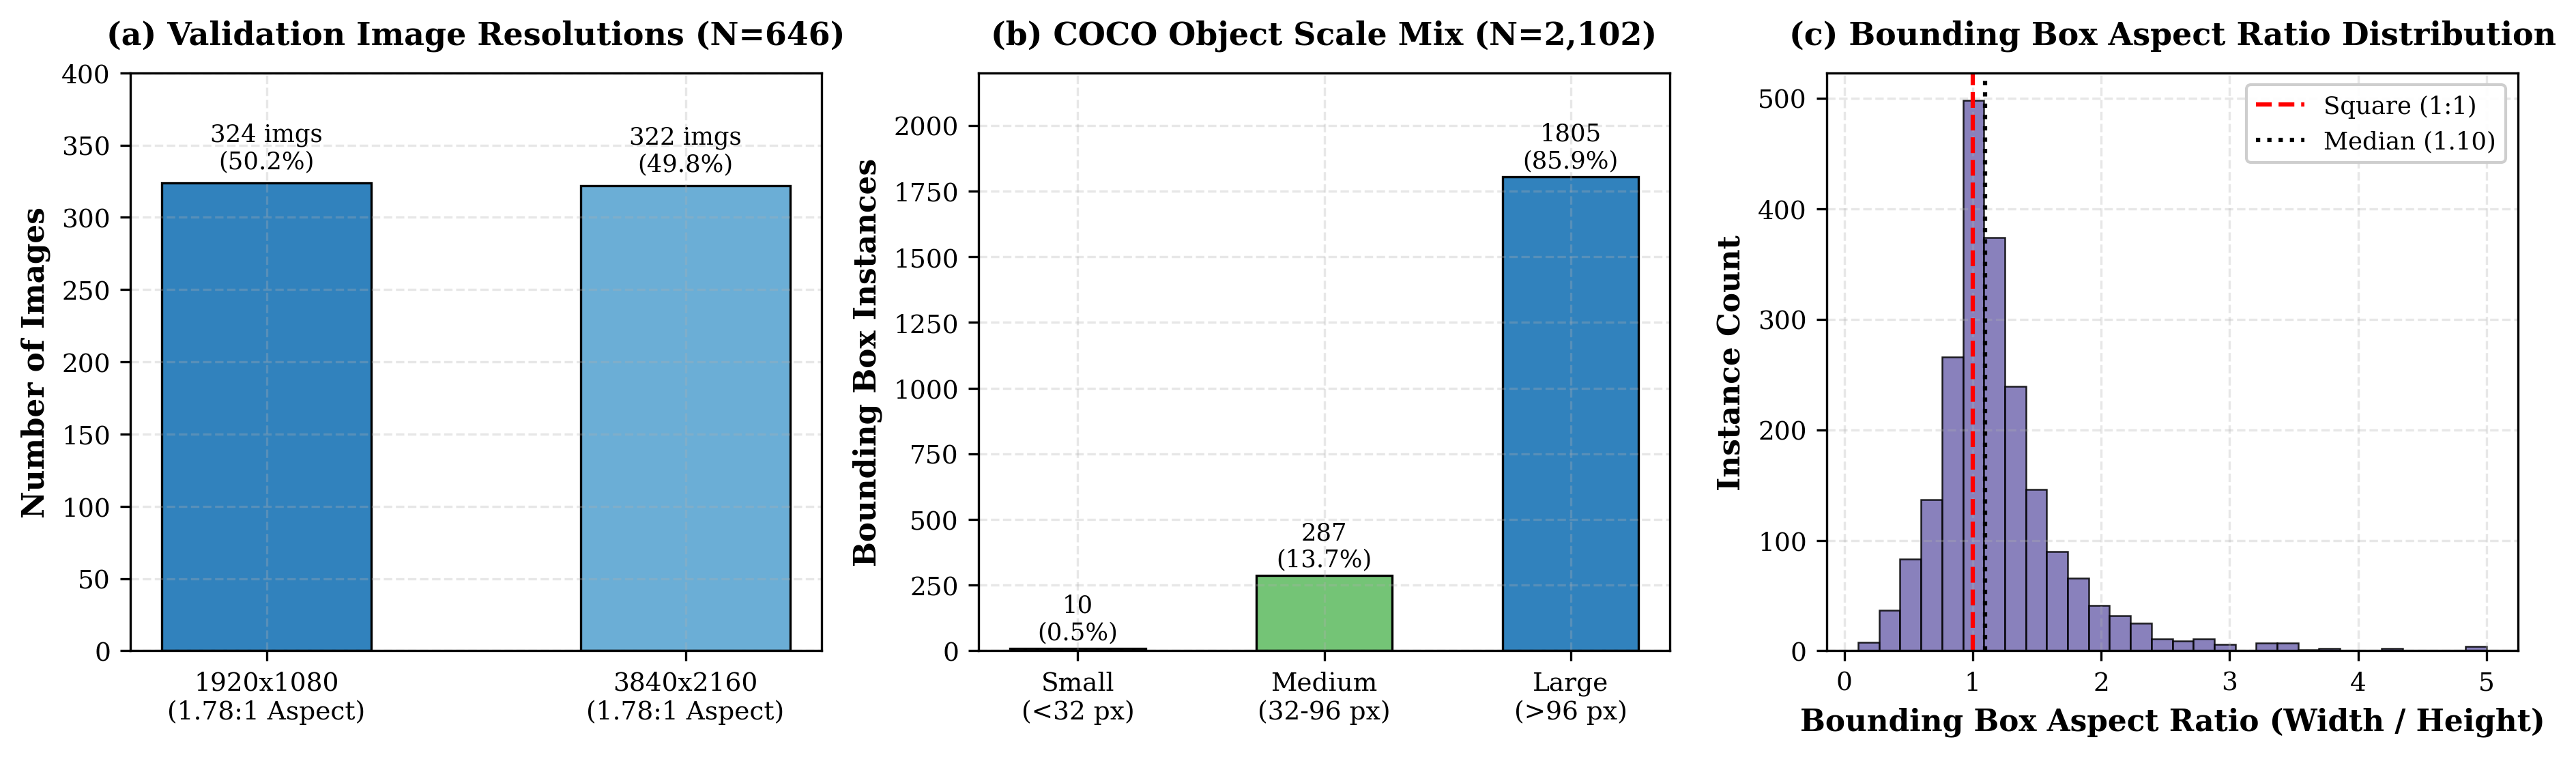
\includegraphics[width=0.98\textwidth]{images/fig_geometry.png}
  \caption{Image and bounding-box geometry audit of the FathomNet CLEF~2026 dataset. (a)~Frame resolution breakdown across validation images, showing 100\% widescreen 16:9 frames evenly split between 1080p ($1920\times 1080$, $50.2\%$) and 4K UHD ($3840\times 2160$, $49.8\%$). (b)~COCO bounding-box scale mix (Small $<32$\,px, Medium $32$--$96$\,px, Large $>96$\,px), indicating that large instances account for $85.9\%$ of annotations, while small objects represent fewer than $0.5\%$ of targets. (c)~Bounding-box aspect ratio distribution ($W/H$), showing concentration around unity (median 1.10) with an extended tail from elongated benthic taxa.}
  \label{fig:eda-geometry}
\end{figure*}

\begin{figure*}[t]
  \centering
  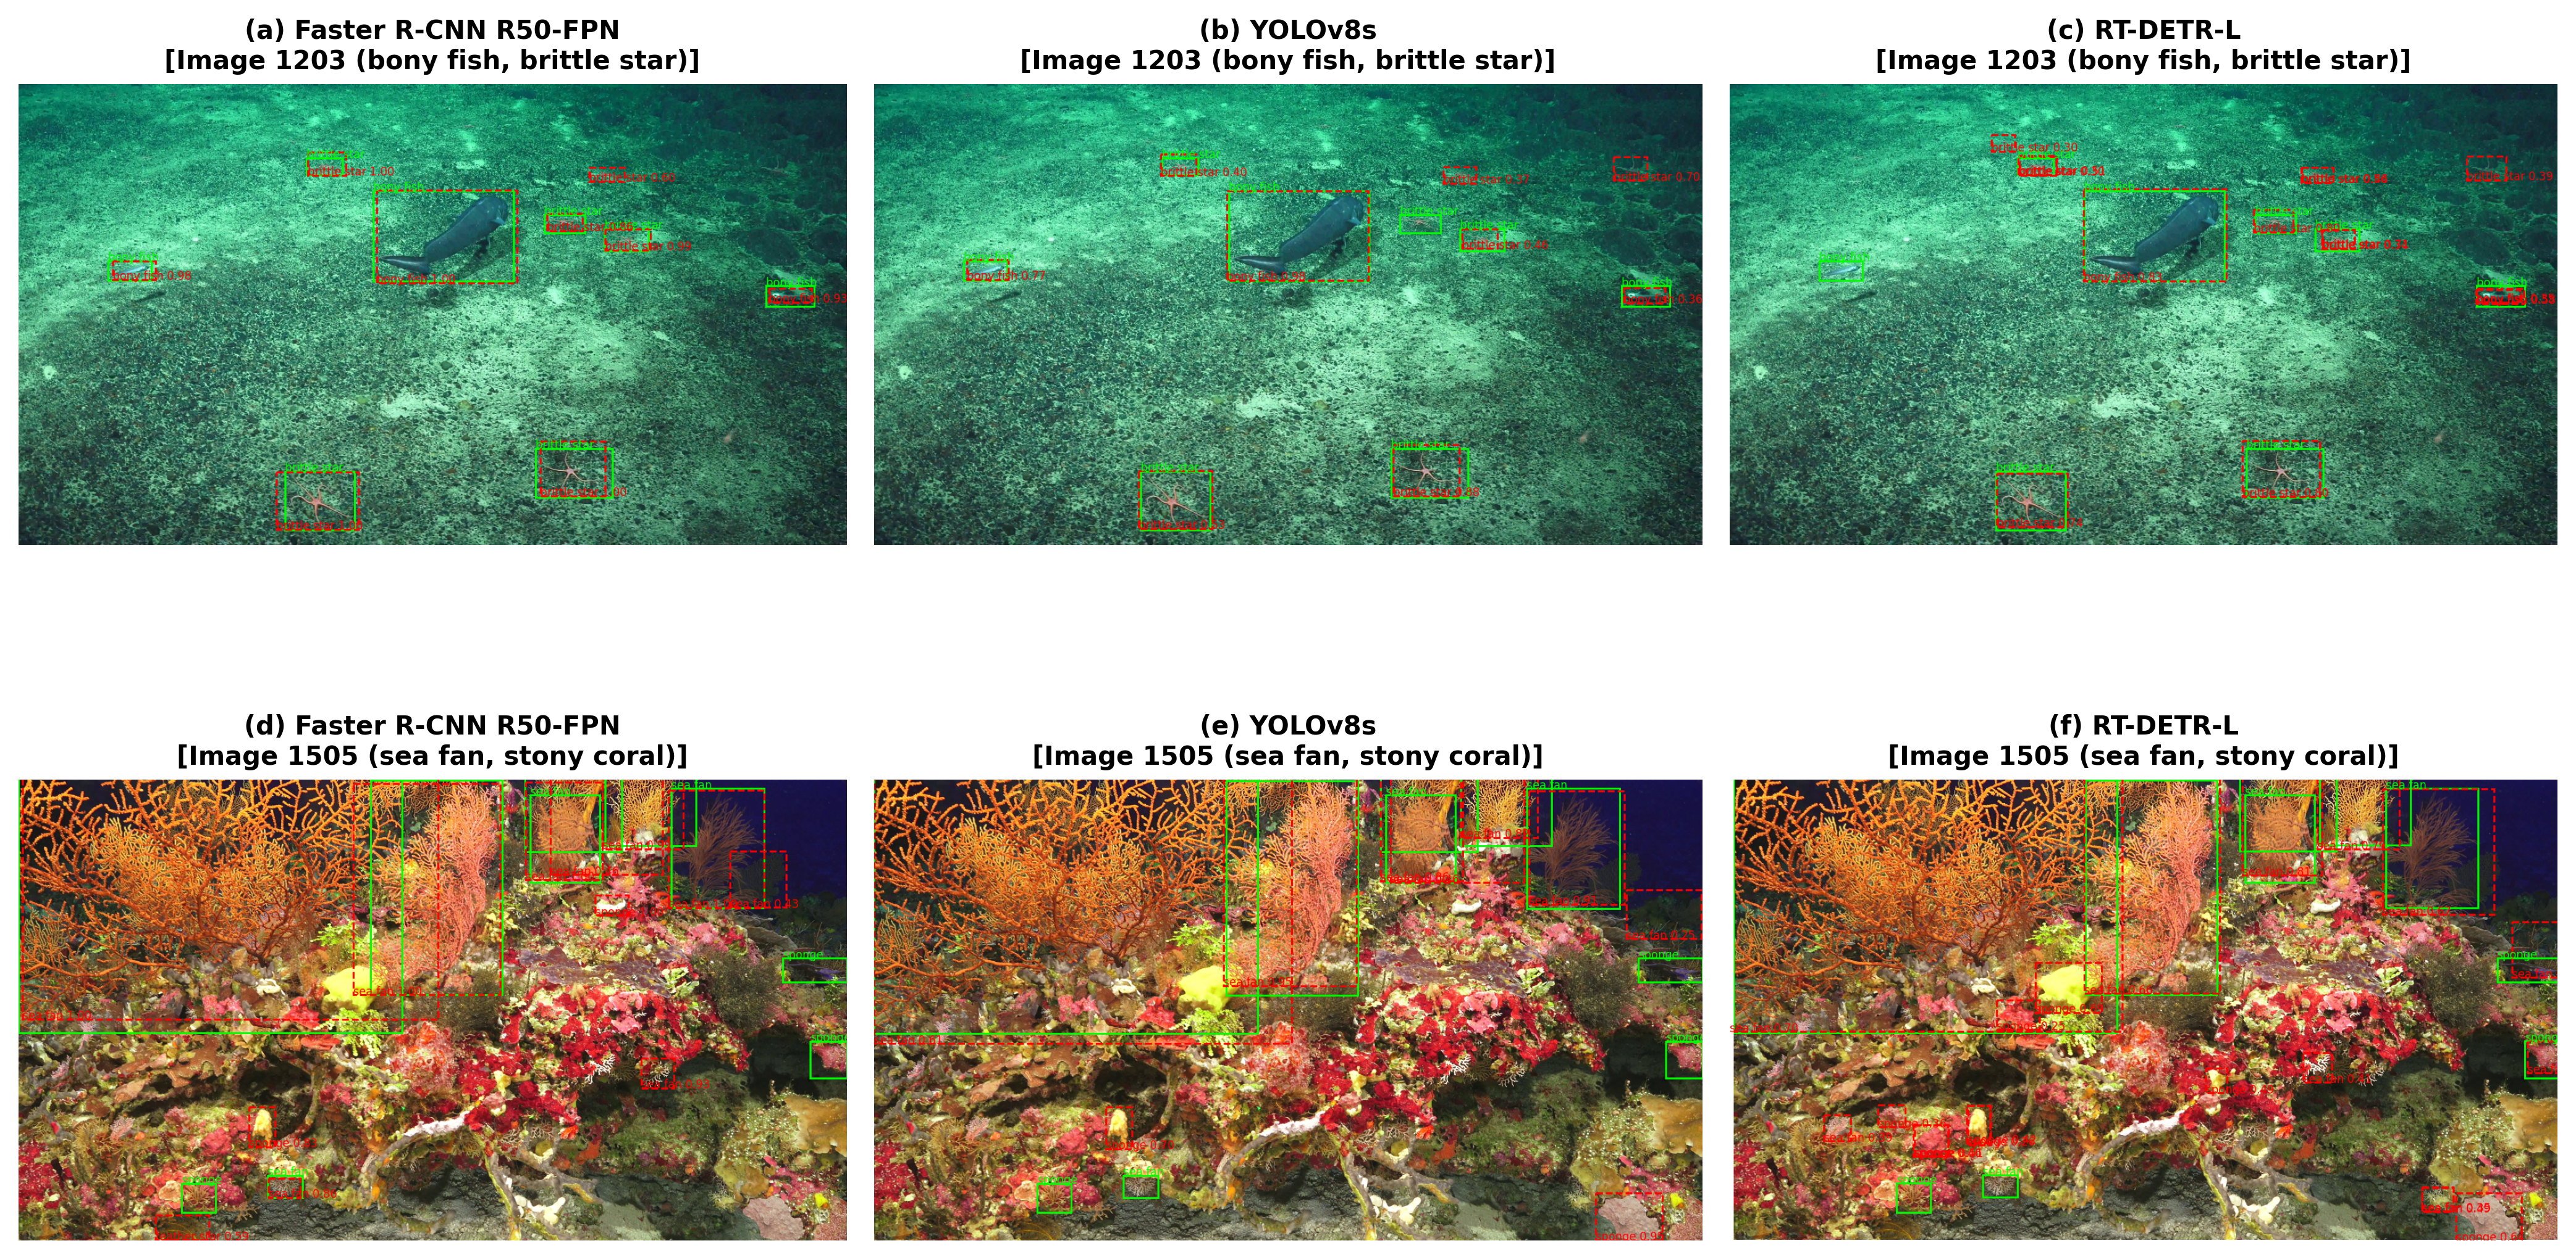
\includegraphics[width=0.98\textwidth]{images/fig_qualitative_large.png}
  \caption{Qualitative detection results on representative benthic validation scenes (Top row: Image 1203 containing \textit{bony fish} and \textit{brittle star}; Bottom row: Image 1505 containing \textit{sea fan} and \textit{stony coral}). Green solid boxes denote ground-truth annotations; red dashed boxes indicate model detections at confidence threshold $\ge 0.25$. Columns compare Faster R-CNN R50-FPN, YOLOv8s, and RT-DETR-L.}
  \label{fig:qualitative}
\end{figure*}

\begin{figure*}[t]
  \centering
  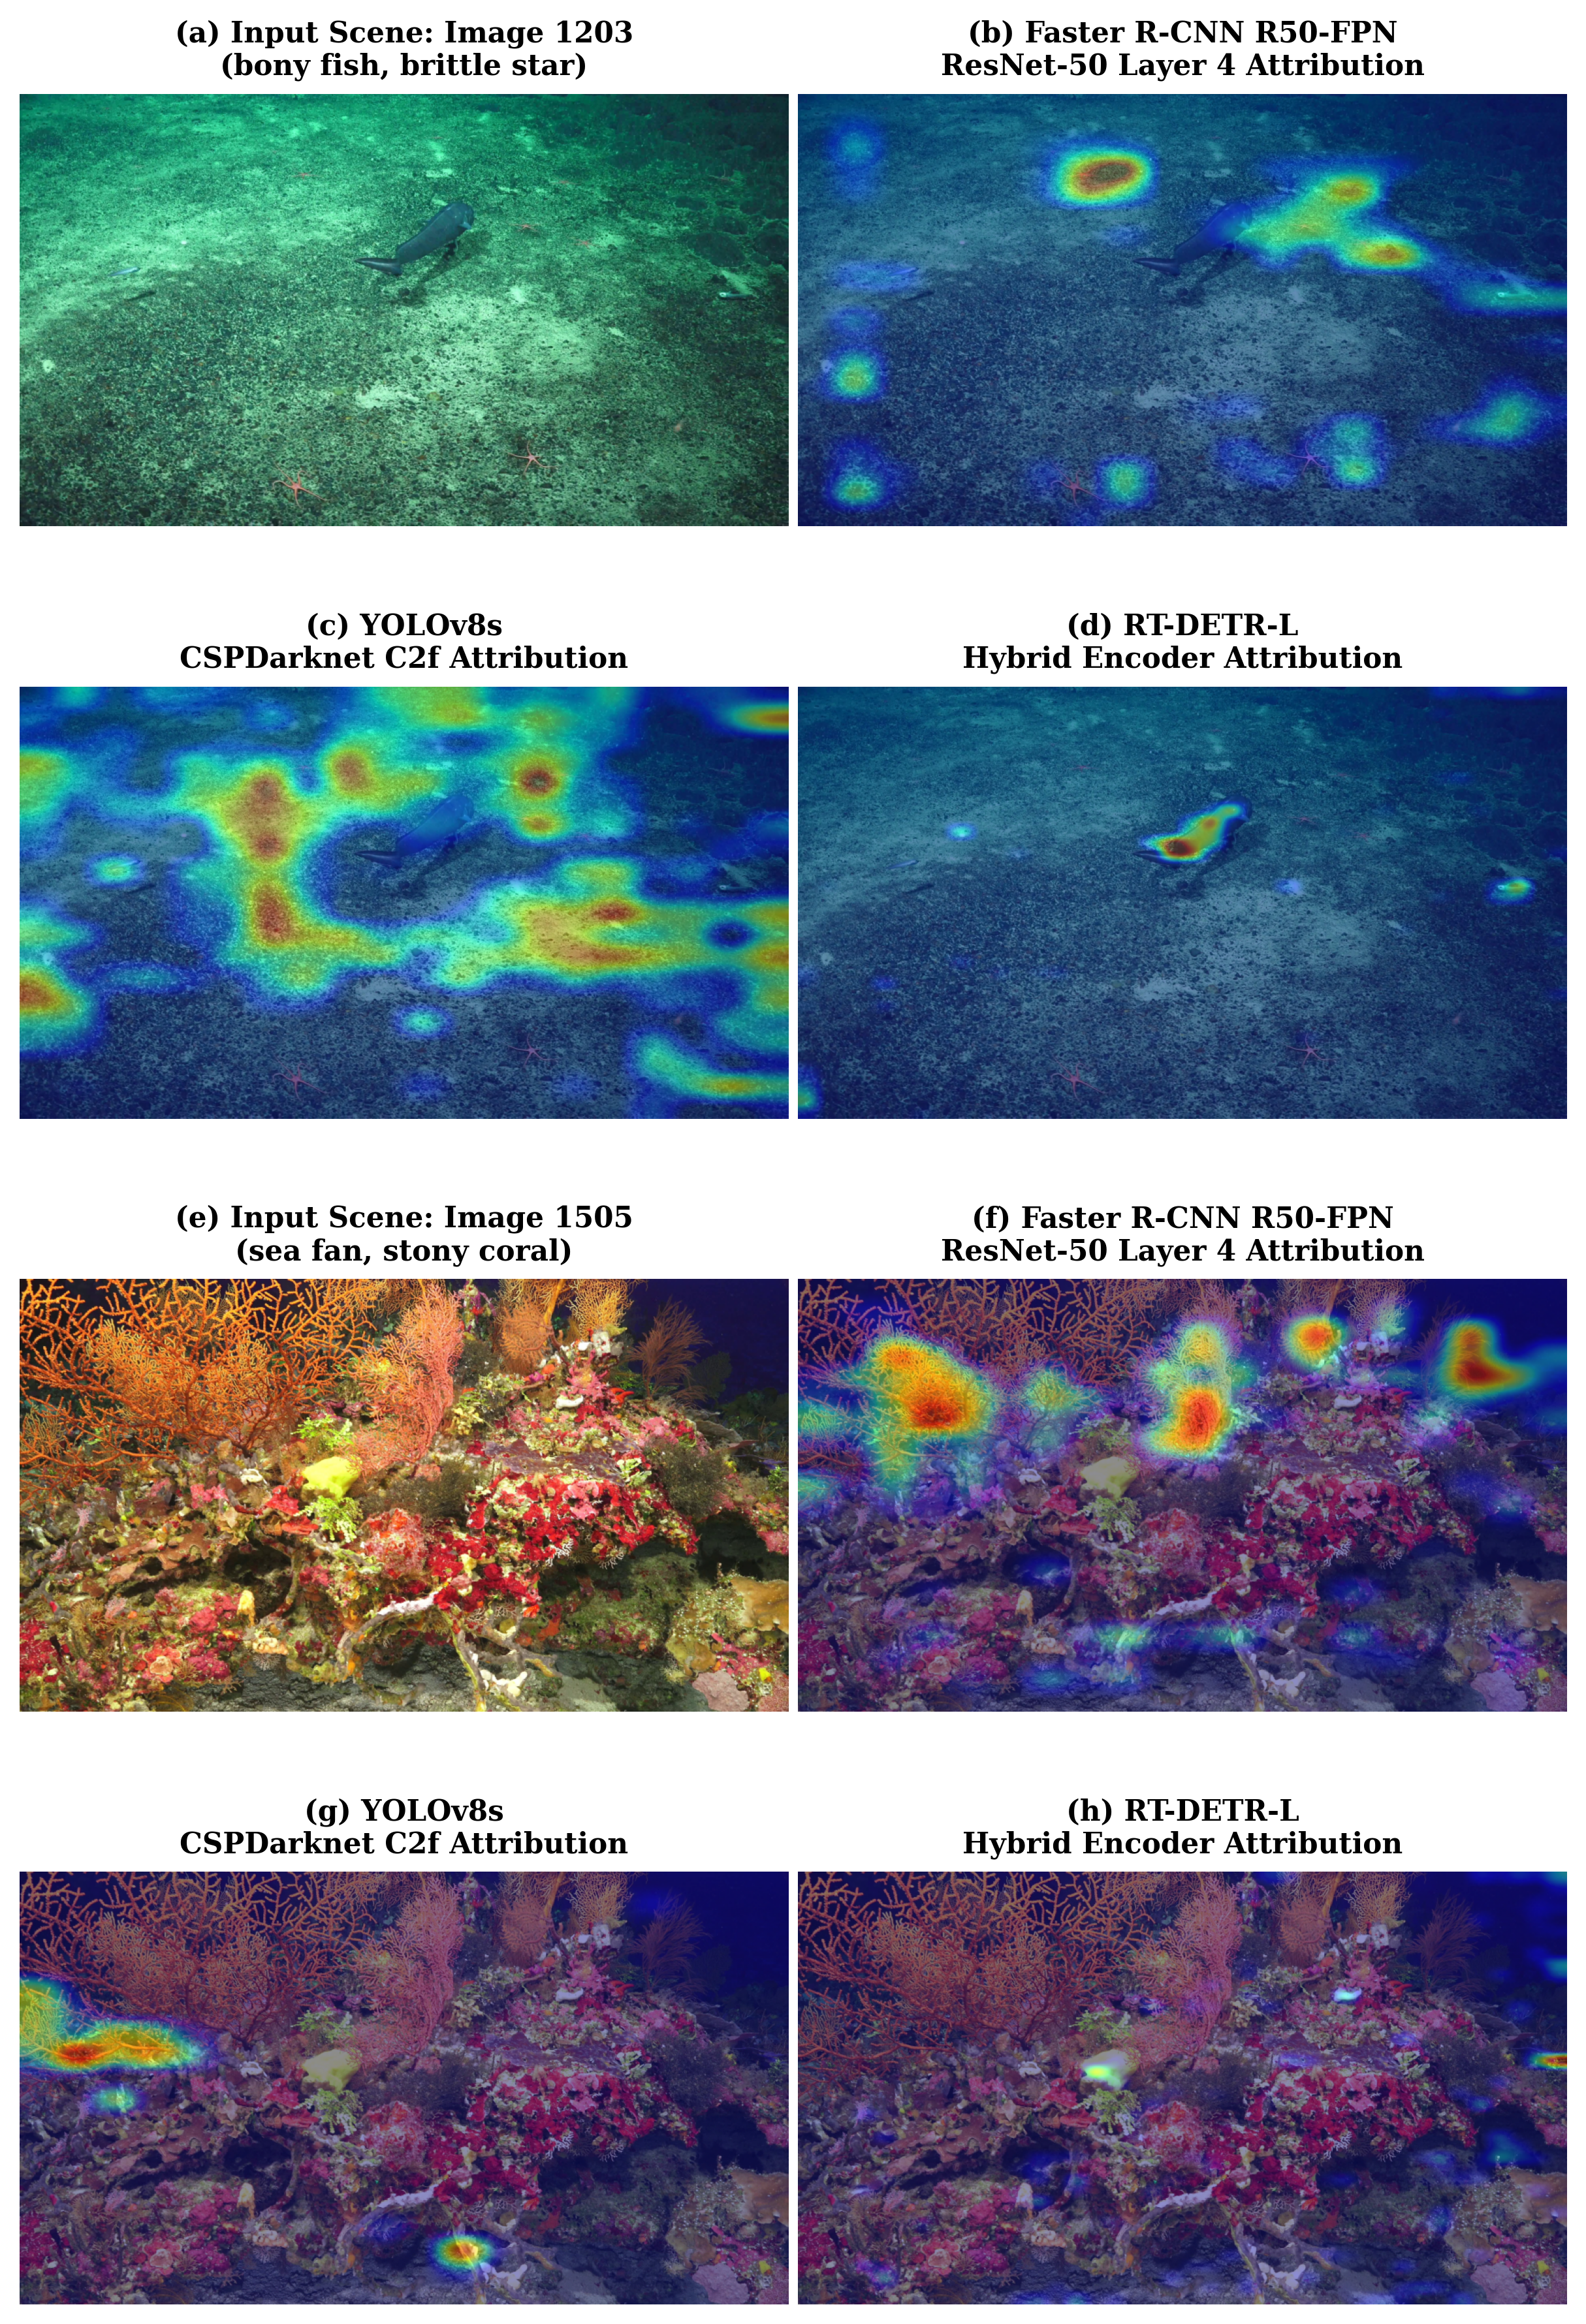
\includegraphics[height=0.66\textheight]{images/fig_gradcam_large.png}
  \caption{High-resolution Grad-CAM visual attributions across architectures on the same validation scenes, arranged as four rows with two panels per row. Rows 1--2 show Image 1203 (target classes: \textit{bony fish}, \textit{brittle star}); rows 3--4 show Image 1505 (target classes: \textit{sea fan}, \textit{stony coral}). For each scene, the input frame is compared against deep layer attributions: ResNet-50 layer 4 for Faster R-CNN, CSPDarknet C2f module for YOLOv8s, and the Hybrid Encoder for RT-DETR-L. Heatmaps highlight precise, localized focal attention for Faster R-CNN in contrast to more diffuse background sensitivity in the one-stage and transformer models.}
  \label{fig:gradcam}
\end{figure*}

\section{Reproducibility and artifact availability}
\label{sec:reproducibility}

The benchmark is fully reproducible using the reproduction suite provided in the
project repository. Execution scripts automate data ingestion, dataset integrity
validation, stratified partitioning, and standardized model training for Faster R-CNN,
YOLOv8s, and RT-DETR-L under identical seed configurations. Each detector run executes
a unified COCO evaluation harness that computes per-class AP and stratum aggregates.
Serialized evaluation metrics, training curves, provenance manifests, and qualitative
visualizations are archived in the repository so that every figure, table, and reported
value in this paper can be audited directly without requiring GPU re-training. All software
environments and library versions are pinned for exact replication.

\clearpage
\nocite{*}
\bibliographystyle{unsrt}
\bibliography{references}
\end{document}
